
% !TEX root = ../YourName-Dissertation.tex

\chapter{Antenna and Antenna Measurement System Development for the Project 8 Experiment}

\section{Introduction}

The FSCD and antenna array CRES represent an innovative approach to beta-decay spectroscopy. While much can be learned from simulations about the systematics of CRES with antenna arrays, laboratory measurements and demonstrations provide critical inputs to sensitivity and simulation models as well as provide a means for calibration and commissioning of the experiment. Therefore, a robust program of antenna and antenna measurement hardware development is important to the success of the FSCD and the development of antenna array CRES more broadly.

In this chapter we summarize the development of an antenna measurement system at Penn State to implement and test the techniques of antenna array CRES on the bench-top, in order to support the efforts of the Project 8 collaboration. In Section \ref{sec:chap4-ant-meas} we provide an introduction to some fundamental parameters and concepts related to antenna measurements as well as an overview of the Penn State antenna measurement system hardware. In Section \ref{sec:SYNCA} we include the manuscript of a paper \cite{p8synca} which details the design and characterization of a specialized antenna developed to mimic the electric fields emitted by an electron in a CRES experiment. This antenna, called the Synthetic Cyclotron Antenna (SYNCA), is intended as a calibration tool for antenna arrays developed for CRES measurements. Lastly, in Section \ref{sec:chap5-fscd-array-measurements} we summarize a set of prototype FSCD antenna array measurements with the SYNCA \cite{p8jugaad}, which we use to validate the simulated performance of the antenna array and estimate systematic errors associated with the antenna array.

\section{Antenna Measurements for CRES experiments}
\label{sec:chap4-ant-meas}

\subsection{Antenna Parameters}
\label{sec:ant-meas-fun}

Antenna characterization measurements are intended to validate simulations of the antenna array performance, which ultimately informs the neutrino mass sensitivity of the experiment. In this section, I shall summarize a few fundamental concepts relating to antennas and antenna measurement, before introducing how Project 8 uses antenna measurement for the development of antenna array CRES.

\subsubsection{Radiation Patterns}

\begin{figure}[htbp]
    \centering
    \begin{subfigure}[b]{0.48\textwidth}
        \centering
        \includegraphics[width=1\textwidth]{figs/Chapter-5/230419_example_radiation_pattern2.png}
        \caption{\label{fig:rad-pattern-ex1}}
    \end{subfigure}
    \hfill
    \begin{subfigure}[b]{0.48\textwidth}
        \centering
        \includegraphics[width=1\textwidth]{figs/Chapter-5/230419_example_radiation_pattern.png}
        \caption{\label{fig:rad-pattern-ex2}}
    \end{subfigure}
    \hfill
    \caption{An example radiation pattern generated using HFSS simulations. The color and radial distance of the surface from the origin indicate the relative magnitude of radiation power emitted by the antenna in that direction. The primary goal of most antenna measurements is typically to measure the antenna pattern, which is used to derive many useful antenna performance parameters.}
    \qquad
    \label{fig:rad-pattern-examples}
\end{figure}

Antennas are conductive structures designed to carry alternating electric currents in order to transmit energy in the form of electro-magnetic (EM) waves \cite{balanis2015antenna}. Perhaps the most fundamental way to characterize an antenna, is to map out the radiated power density as a function of position, which is called the radiation pattern (see Figure \ref{fig:rad-pattern-examples}). We find the radiation power density by calculating the time-averaged Poynting vector for all positions surrounding the antenna, which in equation form is
\begin{equation}
    \mathbf{W}(x,y,z) = \left<\mathbf{E}(x,y,z,t)\times\mathbf{H}^\ast(x,y,z,t)\right>_t,
\end{equation}
where $\mathbf{E}(x,y,z,t)$ and $\mathbf{H}(x,y,z,t)$ are the time-dependent electric and magnetic fields produced by the antenna \cite{jackson_classical_1999}. The radiation power density has units of $\mathrm{W}/\mathrm{m}^2$ and is more typically called the energy flux density in physics applications, since it is a measure of the amount of energy passing through a unit area over time. 

Because the radiation power density is a measure of power per unit area, its value in a particular direction will depend on the distance from the antenna at which we are measuring. This is undesirable for practical applications A related quantity, which is distance independent, is the energy flux per unit solid angle or radiation intensity, which is computed directly from the radition power density by multiplying by the squared distance from the antenna. Specifically,
\begin{equation}
    U = r^2W(x,y,z),
\end{equation}
where $r$ is the distance from the antenna to the field measurement point. The radiation intensity is typically defined in regions where the Poynting vector consists only of a radial component where it is safe to treat as a scalar quantity. 

\subsubsection{Directivity and Gain}
Since the radiation intensity is a measure of average power per unit solid angle, it is independent of distance and more useful as feature for antenna measurement. However, most antenna measurements are performed in terms of the directly related directivity and gain quantities. Directivity is defined as the ratio between the radiation intensity at particular point on the radiation pattern to the average radiation intensity computed over all solid angles \cite{balanis2015antenna}.
The equation that relates the radiation intensity to directivity is
\begin{equation}
    D = \frac{U}{U_0}=\frac{4\pi U}{P_\textrm{rad}},
\end{equation}
where $U_0$ is the average radiation intensity over all solid angles, which simply the total radiated power ($P_\textrm{rad}$) divided by $4\pi$. Closely related to directivity is concept of gain, which accounts for energy losses that occur inside then antenna when attempting to transmit or receive a signal. The antenna gain is given by 
\begin{equation}
    G=\frac{4\pi U}{P_\mathrm{in}},
\end{equation}
where $P_\mathrm{in}$ is the total power delivered to the antenna. Gain can be thought of as the ratio of the antenna's radiation intensity to that of a hypothetical isotropic, lossless radiator. The maximum values of gain and directivity exhibited by the main lobe of the antenna pattern as well as the ratio between the gain of the main lobe and any side-lobes are important figures of merit used to evaluate antenna designs. 

\begin{figure}[htbp]
    \centering
    \includegraphics[width=0.7\textwidth]{figs/Chapter-5/230421_field_regions.png}
    \caption{An illustration of the three field regions important for the analysis of an antenna system. Very close to the antenna the electric fields are primarily reactive so there is no radiation. If a receiving antenna were placed in this region most of the energy would be reflected back to the transmitter. Outside of the reactive near-field is the radiative near field. At these distances the antenna does radiate, but the radiation pattern is not well-defined since it changes based on the distance of the receiving antenna. It is only in the far-field region where the radiation pattern becomes constant as a function of distance, which is where the majority of antenna engineering is assumed to take place. The antenna arrays developed by Project 8 for CRES measurements operate in the radiative near-field due to the importance of limiting power loss from free-space propagation, which complicates the design of the antenna system.}
    \label{fig:field-regions}
\end{figure}

\subsubsection{Far-field and Near-field}
Radiation patterns are only well-defined in regions where the shape of the radiation pattern is independent of distance. The region where this approximation is valid is called the "far-field", and in this region we can treat the EM fields from the antenna as spherical plane waves. A rule of thumb for antennas is that the far-field approximation is valid when the condition
\begin{equation}
    R > \frac{2l^2}{\lambda}
\end{equation}
is met. In this expression, $R$ is the distance from the antenna, $l$ is the largest characteristic dimension of the antenna, and $\lambda$ is the wavelength of the radiation (see Figure \ref{fig:field-regions}). 

The region very close to the antenna is called the reactive near-field, because in this region the reactive component of the EM field is dominant. Unlike radiative electric fields, the reactive electric and magnetic fields are out of phase from each other by $90^\circ$, since they are the result of electrostatic and magnetostatic effects coming from the self-capacitance and self-inductance of the antenna. The reactive fields are unable to transfer energy a significant distance from the antenna and are thus completely negligible for most antenna applications. The limit of the reactive near-field for an electrically-large antenna is typically taken to be
\begin{equation}
    R<0.62\sqrt{l^3/\lambda}.
\end{equation}
The unique application of antennas by Project 8 is somewhat limited by reactive near-field effects in the form of a maximum radial position for electrons inside the uniform cylindrical antenna array. If electrons are too close to the edge of the array than reactive near-field effects leads to a large reduction in the received power and consequently detection efficiency. This leads to a significant volume inside of the antenna array that is unsuitable for CRES lowering the volumetric efficiency of the antenna array CRES technique relative to a cavity experiment.

In between the reactive near-field and the far-field is the radiative near-field region. In this region the fields are primarily radiative, however we are still too close to the antenna for the spherical plane wave approximation to apply. Therefore, interference effects between EM waves emitted from different points on the antenna occur causing the shape of the radiation pattern to change as a function of distance from the antenna. If we evaluate the far-field distance limit for the FSCD one finds an estimated far-field distance of 43~cm, which is a factor of four larger than the radius of the antenna array designed for the experiment. Consequently, we expect near-field effects to influence the performance of the antenna array highlighting the importance of calibration and characterization measurements.

\subsubsection{Polarization}
The polarization of an EM wave defines the spatial orientation of the electric field oscillations in the plane perpendicular to the direction of the propagation, and is defined in terms of orthogonal polarization components. In our application, one analyzes the properties of radiation propagating along the radial ($\hat{r}$) direction away from the antenna, which implies that the electric fields can be described as a linear combination of orthogonal polarization components
\begin{equation}
    \mathbf{E}_\mathrm{tot}=E_x\hat{x}+E_y\hat{y}+E_z\hat{z},
\end{equation}
in Cartesian coordinates, or
\begin{equation}
    \mathbf{E}_\mathrm{tot}=E_\theta\hat{\theta}+E_\phi\hat{\phi},
\end{equation}
in spherical coordinates. 

In general, one defines partial radiation patterns, directivities, and gains so that the performance of the antenna for the desired polarization can be analyzed. The radiation pattern defined in terms of partial patterns is
\begin{equation}
    U_\mathrm{tot}=U_\phi + U_\theta,
\end{equation}
where $U_\phi$ and $U_\theta$ are the radiation intensities in a particular direction for the respective polarization components. Similarly, a quantity such as gain can be written in terms of partial gains,
\begin{equation}
    G_\mathrm{tot}=G_\phi+G_\theta=\frac{2\pi U_\phi}{P_\mathrm{in}}+\frac{2\pi U_\theta}{P_\mathrm{in}}.
\end{equation}

If we view an electron performing a circular orbit in the XY-plane from the side, that is, along the X or Y axes, then we would observe the electron to be performing a linear oscillation perpendicular to the viewing axis. From this intuitive picture, we can predict that the primary polarization of electric fields from CRES events to be linearly polarized in the $\hat\phi$ direction when viewed with an antenna positioned in the XY-plane.

\subsubsection{Antenna Factor and Effective Aperture}
\label{sec:ant-factor}
A useful way to characterize the performance of an antenna is to measure the electric field magnitude required to produce a signal with an amplitude of one volt in the antenna terminals. This ratio between the magnitude of the incoming electric field and the magnitude of the signal produced by the antenna is called the antenna factor, which is written as
\begin{equation}
    A_\mathrm{F} = \frac{|\mathbf{E}_\mathrm{in}|}{V_\mathrm{ant}},
    \label{eq:antenna-factor}
\end{equation}
where $A_\mathrm{F}$ is the antenna factor, $E_\mathrm{in}$ is the incoming electric field, and $V_\mathrm{ant}$ is the magnitude of the voltage produced by the antenna.

The antenna factor can be expressed in terms of the antenna's gain through a related quantity called the effective aperture. The effective aperture defines for a given incident radiation power density ($\mathrm{W}/\mathrm{m}^2$) the power that is received by the antenna. Therefore, the effective aperture gives the equivalent area of the antenna,
\begin{equation}
    A_\mathrm{eff}=\frac{P_\mathrm{rec}}{P_\mathrm{in}}=\frac{\lambda^2}{4\pi}G,
\end{equation}
where the received power is $P_r$ and the total incoming power is $P_\mathrm{in}$.

If we express the incident power in terms of the magnitude of the Poynting vector, then
\begin{equation}
    |\mathbf{S}_\mathrm{in}|=|\mathbf{E}_\mathrm{in}|^2/\eta_0,
\end{equation}
where $\eta_0$ is the impedance of free-space, which relates the magnitudes of the electric and magnetic fields in a vacuum, and is defined by
\begin{equation}
    \eta_0 = \frac{|\mathbf{E}|}{|\mathbf{H}|} = \sqrt{\frac{\epsilon_0}{\mu_0}}.
\end{equation}
The total received power by the antenna can therefore be expressed as
\begin{equation}
    P_\mathrm{rec}=|\mathbf{S}_\mathrm{in}|A_\mathrm{eff}=|\mathbf{S}_\mathrm{in}|\frac{\lambda^2}{4\pi}G=\frac{|\mathbf{E}_\mathrm{in}|^2\lambda^2G}{4\pi\eta_0}.
    \label{eq:power-rec-1}
\end{equation}

To relate this to the antenna factor recall that we can relate the voltage produced by the antenna to the received power with
\begin{equation}
    P_\mathrm{rec}=\frac{V_\mathrm{ant}^2}{Z}=\frac{|\mathbf{E}_\mathrm{in}|^2}{A_\mathrm{F}^2Z},
    \label{eq:power-rec-2}
\end{equation}
where $Z$ is the system impedance. Setting Equations \ref{eq:power-rec-1} and \ref{eq:power-rec-2} equal to each other, we obtain the following expression for antenna factor in terms of gain
\begin{equation}
    A_\mathrm{F} = \sqrt{\frac{4\pi\eta_0}{ZG\lambda^2}}=\frac{9.73}{\lambda\sqrt{G}}.
    \label{eq:ant-factor}
\end{equation}
The second expression in Equation \ref{eq:ant-factor} is obtained by evaluating the constant terms assuming a system impedance of 50~$\Omega$.

We have gone through the effort of expressing the antenna factor in terms of gain to highlight that the majority of antenna parameters that we care to measure for a CRES experiment can be obtained from the radiation or gain pattern of the antenna. The antenna factor is a particularly important parameter for CRES measurements due to it's relevance to antenna array simulations with the Locust software \cite{p8locustpaper, nb_thesis}. Specifically, Locust simulates the trajectory of an electron in a magnetic trap by running the Kassiopeia software package \cite{kassiopeia} and then uses the Li\'{e}nard-Wiechert equations \cite{lw_potential_1, lw_potential_2} to calculate the electric fields that are incident on the antenna. 

To compute the response of the antenna to the electric field, Locust relies upon linear time-invariant system theory \cite{lti_theory_wiki}, which computes the response of the antenna (i.e. the voltage time series generated by the antenna) using a convolution between the electric field time-series and the antenna impulse response. This approach is necessary for correctly modeling the antenna response to the electric field due to the broadband and non-stationary nature of the electric fields from CRES events. Since antenna measurements take place under steady-state conditions, parameters such as the radiation pattern, gain, and antenna factor are defined in the frequency domain. However, by performing an inverse Fourier transform on the antenna factor we can obtain the antenna impulse response, which allows us to simulate CRES events in the antenna array demonstrator experiment. 

\subsection{Antenna Measurement Fundamentals}
\subsubsection{Friis Transmission Equation}

The antenna factor, sometimes called the antenna transfer function, is used to model how the antenna will respond to electric fields emitted from a CRES event. Therefore, being able to measure the antenna transfer function of the antenna array is a key step in the commissioning and calibration phases of an antenna array CRES experiment. A common approach to antenna characterization is to perform a two antenna transmit-receive measurement where an antenna with a known gain is used to characterize the unknown gain of the antenna under test (see Figure \ref{fig:friis-meas}). 
\begin{figure}[htbp]
    \centering
    \includegraphics[width=0.6\textwidth]{figs/Chapter-5/230409_friis_figure.png}
    \caption{An illustration of the Friis measurement technique commonly used for antenna characterization measurements.}
    \label{fig:friis-meas}
\end{figure}

To analyze this two antenna setup we seek to calculate the amount of power from the transmitting antenna that we will detect with the receiving antenna. Using our understanding of antenna gain, we can calculate the power density transmitted by an antenna in a direction $(\theta_t,\phi_t)$ at frequency $f$ and distance $R$, which is given by
\begin{equation}
    w_t = \frac{P_t}{4\pi R^2}G_t(\theta_t,\phi_t,f).
\end{equation}
Here, $P_t$ is the total power delivered to the transmitting antenna and $G_t(\theta_t,\phi_t,f)$ is the value of the transmitting antenna gain. The power density is the power per unit area, so to calculate the total power delivered to the receiving antenna we multiply the transmitted power density by the effective area of the receiving antenna,
\begin{equation}
    P_r = w_tA_{eff,r}=P_t\frac{G_t(\theta_t,\phi_t,f)G_r(\theta_r,\phi_r,f)c^2}{(4\pi Rf)^2},
    \label{eq:friis-eqn}
\end{equation}
where $G_r(\theta_r,\phi_r,f)$ is the gain of the receiving antenna. Equation \ref{eq:friis-eqn} is called the Friis transmission equation \cite{friis_paper,friis_wiki}, which is of fundamental importance for antenna measurements, since it allows one to measure the gain of an unknown antenna by measuring the power received from an antenna with a known gain pattern. Alternatively, if no antenna with a known gain pattern is available, two identical antennas with unknown gain patterns can be used.

\subsubsection{S-Parameters and Network Analyzers}

Instead of directly measuring the power received by the antenna under test, it is more common to measure the ratio of the received power to the transmitted power,
\begin{equation}
    \frac{P_r}{P_t} = \frac{G_t(\theta_t,\phi_t,f)G_r(\theta_r,\phi_r,f)c^2}{(4\pi Rf)^2}.
\end{equation}
This power ratio can be easily measured using a vector network analyzer (VNA), which automates a significant fraction of the measurement process. Network analyzers are used to measure the scattering or S-parameters of a multi-port RF device \cite{pozar}, which describes how waves are scattered between the device ports. The antenna measurements we have been considering can be modeled as a two-port microwave device that we can characterize by measuring how incident voltage waves are transmitted or reflected (see Figure \ref{fig:2port-scattering}).
\begin{figure}[htbp]
    \centering
    \includegraphics[width=0.5\textwidth]{figs/Chapter-5/230429_2port_scattering_figure.png}
    \caption{Illustration of a two-port S-parameter measurement setup. S-parameters characterize how incoming waves of voltage or power scatter of of the RF device under test. This allows you to measure important properties of the device. In particular, we can use this framework to model a two antenna radiation pattern measurement, which we can then automate using a VNA. }
    \label{fig:2port-scattering}
\end{figure}
We can write the scattered waves ($V_1^-$ and $V_2^-$) in terms of the incident ($V_1^+$ and $V_2^+$) waves using the scattering matrix
\begin{equation}
    \begin{pmatrix}
        V_1^-\\
        V_2^-
    \end{pmatrix} = 
    \begin{pmatrix}
        S_{11}&S_{12}\\
        S_{21}&S_{22}
    \end{pmatrix}
    \begin{pmatrix}
        V_1^+\\
        V_2^+
    \end{pmatrix},
\end{equation}
where the elements of the matrix are the device S-parameters. It is assumed that, when exciting the device from a particular port, that all other ports in the network are terminated at the system impedance. This ensures that the incident waves from other ports in the network are zero. Therefore, the S-parameters are the ratios between the scattered and incident waves,
\begin{equation}
    S_{ij} = \frac{V_i^-}{V_j^+}.
\end{equation}
Alternatively, S-parameters can be defined as the ratio of the scattered and incident power, which is proportional to the ratio of the squared voltage waves. Returning to our antenna measurement setup, we see that measuring the ratio of the received to the transmitted power is equivalent to measuring the ratio of power being scattered from port 1 to port 2 in a RF network. Therefore, measuring an antenna's gain can be accomplished quite easily, by using a VNA to perform a two port $S_{21}$ measurement.

\subsubsection{Antenna Array Commissioning and Calibration Measurements}

Up to this point we have been discussing calibration and commissioning measurements as they apply to a single antenna. While these measurements play an important role in validating the radiation patterns of the individual array elements, the ultimate goal is to use a phased array of these antennas. Therefore, we must also consider antenna measurement techniques that apply to the whole array system.
\begin{figure}[htbp]
    \centering
    \begin{subfigure}[b]{0.4\textwidth}
        \centering
        \includegraphics[width=1\textwidth]{figs/Chapter-5/230409_beamform_array_meas.png}
        \caption{\label{fig:beam-array-meas}}
    \end{subfigure}
    \hfill
    \begin{subfigure}[b]{0.4\textwidth}
        \centering
        \includegraphics[width=1\textwidth]{figs/Chapter-5/230409_beamform_synth_array_meas.png}
        \caption{\label{fig:beam-synth-array-meas}}
    \end{subfigure}
    \hfill
    \caption{Two measurement approaches to characterizing an antenna array for CRES measurements. The full-array approach (a) requires a complete antenna array with all the associated hardware. The synthetic array approach (b) utilizes a single antenna and a set of rotation/translation stages to reposition the transmitter or the recieing antenna to synthesize the signals that would be received by the full-array. This approach reduces the cost and complexity of array measurements. A down-side of the synthetic array approach is that multi-channel effects such as reflections cannot be measured. Utilizing both the full-array and the synthetic array is a powerful way to quantify the impact of errors from the multi-channel array.}
    \qquad
    \label{fig:array-measurements}
\end{figure}

By measuring the gain of each individual array element we can predict the features of the signals received during a CRES event using the antenna factor (see Section \ref{sec:ant-factor}). However, unpredictable changes to the antenna performance can be introduced by the incorporation of the antennas into the circular array geometry, therefore, we employ both individual antenna and full-array measurements in the commissioning of the FSCD to account for these effects.

There are two main approaches to array measurements that could be used for characterization and calibration (see Figure \ref{fig:array-measurements}). One approach is to construct the complete array and use a omni-directional transmitting antenna to measure the power received by each channel in the antenna array. In Section \ref{sec:SYNCA} we describe the development of an omni-directional transmitter that also mimics the radiation phase characteristics of a CRES event, which is useful because the entire array can be tested without repositioning. Alternatively, a full antenna array can by synthesized by repeatedly moving and measuring a single array element. This approach is ideal for identifying if different channels in the antenna array are affecting each other through multi-path interference by comparing the measurement results of the synthetic array to the real array. 

\subsection{The Penn State Antenna Measurement System}
\label{sec:antenna_measurement_system}

The development of antenna array based CRES requires the capability to test and calibrate different antenna array designs to validate the performance of the as-built antenna array before and during the experiment. With these aims in mind we developed an antenna measurement system at Penn State specifically designed to mimic the characteristics of the antenna experiment designed for demonstration of the antenna array CRES technique by the Project 8 collaboration. 

The Penn State antenna measurement system utilizes a two antenna measurement configuration with a stationary reference antenna and a test antenna mounted on a set of motorized translation and rotation stages (see Figure \ref{fig:meas-sys-cartoon}). The antenna measurement system can be operated in two distinct modes, one focused on the characterization of the radiation patterns of prototype antennas and the other focused on the validation of data-acquisition (DAQ) and CRES signal reconstruction techniques to bridge the gap between real measurements and simulation. In both measurement configurations it is critical to isolate the antennas from the environment so that multi-path reflections do not negatively influence the measurement results. For this reason we surround the measurement volume with microwave absorber foam (AEMI AEC-1.5) \cite{absorber_foam} specifically designed to attenuate microwave radiation near the 26 GHz measurement range of the system.

\begin{figure}[htbp]
    \centering
    \includegraphics[width=0.5\textwidth]{figs/Chapter-5/230409_measurement_system_figure_cartoon.png}
    \caption{Illustration of the antenna measurement system developed for the Project 8 Collaboration. The reference and test antennas can be connected to different data acquisition configurations depending on the measurement goals The reference antenna is typically a standard horn antenna and the test antenna is mounted on a set of translation stages for positioning. Automated translation stages allows for relatively painless data-taking enabling synthetic antenna array measurements using only a single receiving antenna. Anechoic form designed to mitigate RF reflections surrounds the setup.}
    \label{fig:meas-sys-cartoon}
\end{figure}

In the first measurement configuration the reference antenna is typically a well-characterized horn antenna as pictured, since horn antennas have well-known and stable radiation patterns making them ideal as standard references. For characterization measurements, the test antenna represents the antenna-under-test whose pattern we wish to characterize. Mounting the test antenna on motorized rotation and translation stages allows us to automate the procedure significantly speeding up the radiation pattern measurement process. 

In the second measurement configuration one is interested in recreating the conditions of an antenna array CRES experiment as it concerns the antenna array and DAQ system. In this case, the reference antenna is a prototype FSCD antenna, which will be used to construct the antenna array in the FSCD experiment, and the test antenna is a specially designed synthetic cyclotron antenna (SYNCA) as picture in Figure \ref{fig:meas-sys-cartoon}. The SYNCA is designed such that the radiation pattern mimics that of a CRES electron so that the signals received by the prototype CRES array antenna mimic what is expected for a real CRES experiment. 

%\subsection{Antenna Measurement Hardware}

\begin{figure}[htbp]
    \centering
    \begin{subfigure}[b]{0.43\textwidth}
        \centering
        \includegraphics[width=1\textwidth]{figs/Chapter-5/230409_vna_sys_diag.png}
        \caption{\label{fig:vna-meas-sys}}
    \end{subfigure}
    \hfill
    \begin{subfigure}[b]{0.52\textwidth}
        \centering
        \includegraphics[width=1\textwidth]{figs/Chapter-5/230408_detail_meas_sys_diag.png}
        \caption{\label{fig:dig-meas-sys}}
    \end{subfigure}
    \hfill
    \caption{\label{fig:meas-sys-diagrams}Diagrams of two measurement system configurations. Configuration (a) utilizes a VNA and is more suited to antenna characterization. Configuration (b) utilizes an AWG and VNA as a signal generation system and digitizer to collect measurement data, which is more suited to simulating CRES measurements. The transmission chain utilizes a quadrature hybrid and a pair of baluns to drive the cross-dipole variant test antenna developed for synthetic CRES measurements.}
\end{figure}

In Figure \ref{fig:meas-sys-diagrams} we show two high-level system diagrams of the Penn State antenna measurement system that depict the important system components and the connections between them. The two configurations of the measurement system utilize different hardware. For characterization and radiation pattern measurements, one prefers the configuration shown in Figure \ref{fig:vna-meas-sys}. In this case a vector network analyzer (VNA) is used as both the transmission source and data acquisition system and it is relatively easy to calibrate over a wide range of frequencies. Whereas, if one is more interested in recreating what would take place in the FSCD experiment then the configuration shown in Figure \ref{fig:dig-meas-sys} is preferable, since this system effectively mimics the receiver chain envisioned for the FSCD experiment. 

The characterization configuration utilizes a network analyzer (Keysight N5222A) \cite{vna, keysight_vna} with two independent sources and four measurement ports as the primary measurement tool. A standard reference antenna is connected to one measurement port, and the test antenna is connected to a separate port. The typical reference antenna used for these studies is a Pasternack PF9851 horn antenna \cite{pasternack_antenna}. In the measurement shown, the test antenna represents a SYNCA antenna, which requires a transmission chain consisting of quadrature hybrid coupler \cite{marki, quad} (Marki QH-0226) connected to two baluns \cite{balun} (Marki BAL-0026) to generate feed signals with the appropriate phases. The VNA measures the radiation pattern by performing a transmission S-parameter measurement, which can be used with the knowledge of the reference antenna's radiation pattern to determine the radiation pattern of the test antenna (see Section \ref{sec:ant-meas-fun}).

The second configuration is more complicated and incorporates more hardware components in order to more closely mimic the DAQ system envisioned for the FSCD experiment. The basic approach is to produce CRES-like radiation and use an antenna combined with a realistic RF receiver chain to acquire the signals. On the transmit side, an arbitrary waveform generator  \cite{awg} (AWG, RIGOL DG5252) is used to generate a waveform that mimics a CRES signal at a baseband frequency up to 250~MHz. This frequency is then up-converted to the CRES signal frequency band of 25.8 to 26.0 GHz using a mixer \cite{mixer} (Marki MM1-0832L) and a bandpass filter (K\&L Microwave 3C62-25900/T200-K/K) to reject unwanted mixing components outside out of the 200~MHz CRES signal band. The local oscillator signal for mixing is provided by one of the VNA sources configured to run in a continuous wave setting. On the receive side, a prototype antenna is used to detect the radiation emitted by the test antenna, which is down-converted and filtered using the same mixer and bandpass filter as the transmission chain. Lastly, data acquisition is performed using a 14-bit ADC sampling at 500~MSa/s \cite{caen} (CAEN DT530) to digitize the down-converted signals.

In order to distribute the LO to all mixers a 4-way power splitter (MiniCircuits ZC4PD-18263-S+) along with an amplifier (Marki APM-6848) is used to drive the four mixers used in the measurement system. A limitation of using the VNA as an LO source is that there is no control of the LO phase when a measurement is triggered by the control script, which leads to a random phase offset between acquisitions. This makes it impossible to perform synthetic array measurements, which require strict control over the starting phase of the transmitted signal. In order to monitor the random phase of the LO, a 2-way power splitter (MiniCircuits Z99SC-62-S+) is used to split the signal from the AWG between the transmission path and a LO monitoring path. The LO monitoring path consists of an up-conversion and down conversion using two mixers connected by a coaxial cable, and monitors the relative phase of the LO using a channel on the digitizer to sample this path. A phase shift in the LO will lead to a proportional phase shift in the mixed signal, which is measured and removed from the received signals.

The test antenna is mounted on a set of motorized stages, which are identical for both measurement configurations. A rotational stage (ThorLabs PRMTZ8) is used as the base layer with additional translation stages mounted on top of this. The rotational stage is ideal for measuring a complete azimuthal scan of the test antenna's radiation pattern as well as for moving a SYNCA antenna in circular motion to recreate the symmetry of the FSCD antenna array. On top of the rotational stage we mount two linear translation stages (ThorLabs MTS50-Z8 and MTS25-Z8) in a cross-wise manner so that the test antenna can be moved along two perpendicular axes. Using the linear stages in combination with the rotational stage allows one to fine-tune the positioning of the test antenna so that it can be perfectly aligned with the central axis of the array. A LabView script was developed to automate the measurement of a full $360^\circ$ radiation pattern and control the measurement electronics. Data from these acquisitions is stored on university provided cloud storage.

\section{Development of a Synthetic Cyclotron Antenna (SYNCA) for Antenna Array Calibration}
\label{sec:SYNCA}
This section is the manuscript of the publication \cite{p8synca} detailing the development of a Synthetic Cyclotron Antenna (SYNCA) for antenna array characterization measurements by the Project 8 collaboration. 

\subsection{Introduction}
\label{sec:intro}

Neutrinos are the most abundant standard model fermions in our universe, but due to weak interaction cross-sections with other particles, neutrinos are particularly difficult to study. Consequently, many fundamental properties of neutrinos are still unknown including the absolute scale of the neutrino mass \cite{Workman:2022ynf}. Direct, kinematic measurements of the neutrino mass are particularly valuable due to their model independent nature \cite{FORMAGGIO20211}. To date the most sensitive direct neutrino mass measurements have been performed by the KATRIN collaboration \cite{Aker2022}, which measures the molecular tritium $\beta$-decay spectrum to infer the neutrino mass. Current data from neutrino oscillation measurements \cite{Workman:2022ynf} allow for neutrino masses significantly smaller than the design sensitivity of the KATRIN experiment; therefore, there is a need for new technologies for performing direct neutrino mass measurements to probe lower neutrino masses.

\begin{figure}[htbp]
\centering
\includegraphics[width=.6\textwidth]{figs/Chapter-5/220914_fscd_cartoon.pdf}
\qquad
\caption{\label{fig:fscd-cartoon} A sketch of an antenna array large-volume CRES experiment. Electrons from $\beta$-decays are confined in a magnetic field using a set of trap coils. The cyclotron radiation produced by the motion of the trapped electrons can be detected by a surrounding antenna array to determine the electron energies. Measuring the energies of many electrons produces a $\beta$-decay spectrum.}
\end{figure}

The Project 8 collaboration is developing new methods for neutrino mass measurement based on Cyclotron Radiation Emission Spectroscopy (CRES) \cite{Monreal:2009za, Project8:2014ivu, Project8:2017nal, Project8:2022wqh}, with the goal of measuring the absolute scale of the neutrino mass with a 40 $\textrm{meV}/\textrm{c}^2$ sensitivity \cite{PhysRevC.103.065501, FORMAGGIO20211}. This sensitivity goal will require the development of two separate technical capabilities. First is the development of an atomic tritium source, which avoids significant spectral broadening due to molecular final states \cite{Bodine:2015sma}. Second is the technology for performing CRES in a multi-cubic-meter experimental volume with high combined detection and reconstruction efficiency, which is required in order to obtain sufficient event statistics near the tritium spectrum endpoint.

One approach for a large-volume CRES experiment is to use an array of antennas, which surrounds a volume of tritium gas, to detect the cyclotron radiation produced by the $\beta$-decay electrons when they are trapped in a background magnetic field using a set of magnetic trapping coils (see Figure \ref{fig:fscd-cartoon}). Project 8 has developed a conceptual experiment design to study the feasibility of this approach. The design consists of a single circular array of antennas with a radius of 10~cm and 60 independent channels positioned around the center of the magnetic trap. The motivation behind this antenna array design is to first develop an understanding of the antenna array approach to CRES with a small scale experiment before attempting to scale the technique to large volumes by using multiple antenna rings to construct the full cylindrical array. The development of the antenna array approach to CRES has largely proceeded through simulations using the Locust software package \cite{Ashtari_Esfahani_2019, nb_thesis}, which is used to model the fields emitted by CRES events and predict the signals received by the surrounding antenna array. To validate these simulations, a dedicated test stand is being constructed to perform characterization measurements of the prototype antenna array developed by Project 8 (see Figure \ref{fig:testbed-cartoon}) and benchmark signal reconstruction methods using a specially designed transmitting calibration probe antenna.
\begin{figure}[htbp]
\centering
\includegraphics[width=.4\textwidth]{figs/Chapter-5/220726_synca_measurements.pdf}
\qquad
\caption{\label{fig:testbed-cartoon} A schematic of the antenna array test stand. The circular antenna array has a radius of 10~cm with 60 independent channels (limited number shown for clarity). The test stand includes an arbitrary waveform generator (AWG), local oscillator (LO), and data acquisition (DAQ) hardware. Finally, a specialized Synthetic Cyclotron Antenna (SYNCA) is used to inject signals to test the antenna array.}
\end{figure}

We call this probe antenna the Synthetic Cyclotron Antenna or SYNCA. The SYNCA is a novel antenna design that mimics the cyclotron radiation generated by individual charged particles trapped in a magnetic field, which will be used in the antenna test stand to perform characterization measurements, simulation validation, and reconstruction benchmarking. This paper provides an overview of the design, construction, and characterization measurements of the SYNCA performed in preparation for its usage as a transmitting calibration probe. 

In Section \ref{sec:pheno} we provide a description of the cyclotron radiation field characteristics that we recreate with the SYNCA. In Section \ref{sec:synca_design} we give an overview of the simulations performed to develop an antenna design that mimics the characteristics of cyclotron radiation. In Section \ref{sec:synca-characterization-meas} we outline characterization measurements to validate that the fields generated by the SYNCA match simulation, and finally in Section \ref{sec:synca-beamforming-meas} we demonstrate an application of the SYNCA to test phased array reconstruction techniques on the bench-top.

\subsection{Cyclotron Radiation Phenomenology}
\label{sec:pheno}

To understand the cyclotron radiation phenomenology that the SYNCA should mimic, we consider a charged particle moving at relativistic speed in the presence of an external magnetic field (see Figure \ref{fig:physics-situation}). In the special case we shall examine, the entirety of the electron's momentum is directed perpendicular to the magnetic field; therefore, the trajectory of the electron is confined to the cyclotron orbit plane. Because the momentum vector is oriented perpendicular to the magnetic field, electrons with these trajectories are said to have pitch angles of $90^\circ$. 

\begin{figure}[htbp]
\centering
\includegraphics[width=.5\textwidth]{figs/Chapter-5/221012_physical_situation.pdf}
\qquad
\caption{\label{fig:physics-situation} An electron (red dot) performing cyclotron motion in the x-y plane. The resulting cyclotron radiation is observed by an antenna located at the field point of interest. }
\end{figure}

The cyclotron radiation fields generated by this circular trajectory are those which we aim to reproduce with the SYNCA. We can describe the electromagnetic (EM) fields using the Li\'{e}nard-Wiechert equations \cite{jackson_classical_1999, nb_thesis}, which in non-covariant form express the electric field as
\begin{equation}
    \label{eq:lw-e}
      \vec{E}  =e\left[\frac{\hat{n}-\vec{\beta}}{\gamma^2(1-\vec{\beta}\cdot\hat{n})^3|\vec{R}|^2}\right]_{t_\textrm{r}}
      +\frac{e}{c}\left[\frac{\hat{n}\times[(\hat{n}-\vec{\beta})\times\dot{\vec{\beta}}]}{(1-\vec{\beta}\cdot\hat{n})^3|\vec{R}|}\right]_{t_\textrm{r}},
\end{equation}
where $e$ is the particle's charge, $\hat n = (\vec{r}-\vec{r_s})/|\vec{r}-\vec{r_s}|$ is the unit vector pointing from the electron to the field measurement point, $\vec\beta=\dot{\vec{r_s}}/c$ is the velocity of the particle divided by the speed of light, and $\gamma$ is the relativistic Lorentz factor. The equation is meant to be evaluated at the retarded time as indicated by $t_\textrm{r}=t-|\vec{R}|/c$, which accounts for the time delay due to the finite speed of light between the point where the field was emitted and the point where the field is detected.

We would like to simplify Equation \ref{eq:lw-e} it at all possible. As a first step we analyze the relative magnitudes of the electric field polarization components. Consider an electron following a circular cyclotron orbit in a uniform magnetic field whose guiding center is positioned at the origin of the coordinate system. The equation of motion can be expressed as 
\begin{equation}
    \vec r_s= (r_c\cos{\omega_ct_{r}})\hat x+(r_c\sin{\omega_ct_{r}})\hat y.
\end{equation}
For single antenna located along the y-axis at position $\vec{r}=r_{a}\hat{y}$ we are interested in the incident electric fields from the electron. The electric field is given by Equation \ref{eq:lw-e}, which we evaluate in the regime where $r_{a}\gg r_c$. This limit can justified by comparing the radius of the cyclotron orbit for an electron with the tritium beta-spectrum endpoint energy of 18.6~keV in a 1~T magnetic field to the typical ($r_{a}\simeq100$~mm) radial position of the receiving antenna. We find that the cyclotron orbit has a radius of 0.46~mm which is approximately a factor of 200 smaller than the typical antenna radial position. In this regime we can make the approximation $\vec{R}\simeq r_{a}\hat{y}$ and the expression for the electric field at the antenna's position becomes
\begin{multline}
    \label{eq:lw-xy-comp}
    \vec{E}=\frac{e}{\gamma^2r_{a}^2}\frac{\hat{x}(\frac{r_c\omega_c}{c}\sin{\omega_ct_{r}})+\hat{y}(1-\frac{r_c\omega_c}{c}\cos{\omega_ct_{r}})}{(1-\frac{r_c\omega_c}{c}\cos{\omega_ct_{r}})^3}
    - \frac{e}{cr_{a}}\frac{\hat{x}(\frac{r_c^2\omega_c^3}{c^2}-\frac{r_c\omega_c^2}{c}\cos{\omega_ct_{r}})}{(1-\frac{r_c\omega_c}{c}\cos{\omega_ct_{r}})^3}.
\end{multline}
Since the receiving antenna is part of a circular array of antennas, it is useful to rewrite Equation \ref{eq:lw-xy-comp} in terms of the azimuthal ($\hat{\phi}$) and radial ($\hat{r}$) polarizations. Making use of the fact that for an antenna located at $R=r_{a}\hat{y}$ that $\hat{\phi}=-\hat{x}$ and $\hat{r}=\hat{y}$ we find
\begin{align}
    \vec{E}&=\hat{\phi}E_\phi+\hat{r}E_r\\
    \label{eq:e-field-azimuthal-comp}
    E_\phi&=\frac{e}{(1-\frac{r_c\omega_c}{c}\cos{\omega_ct_{r}})^3}\left[-\frac{\frac{r_c\omega_c}{c}\sin{\omega_ct_{r}}}{\gamma^2r_{a}^2}+\frac{\omega_c\left(\frac{r_c^2\omega_c^2}{c^2}-\frac{r_c\omega_c}{c}\cos{\omega_ct_{r}}\right)}{cr_{a}}\right]\\
    E_r&=\frac{e(1-\frac{r_c\omega_c}{c}\sin{\omega_ct_{r}})}{\gamma^2r_{a}^2(1-\frac{r_c\omega_c}{c}\cos{\omega_ct_{r}})^3}.
\end{align}

For the purposes of designing a synthetic cyclotron radiation antenna we are interested in the dominant electric field polarization emitted by the electron. The antenna is being designed to mimic the cyclotron radiation produced by electrons with kinetic energies of approximately 18.6~keV in a 1~T magnetic field \cite{Bodine:2015sma}. Since the relativistic beta factor for an electron with this kinetic energy is  $|\vec{\beta}|\simeq\frac{1}{4}$, the approximations $\gamma\simeq1$ and $\frac{r_c\omega_c}{c}\simeq\frac{1}{4}$ are justified. Inserting these expressions into the equations for the electric field components above simplifies the comparison of the magnitudes of the two components. Additionally, we compare the time-averaged magnitudes to evaluate the root mean squared electric field ratio. The time-averaged ratio of the radial and azimuthally polarizied electric fields with the above simplifications is given by
\begin{equation}
    \label{eq:e-field-ratio}
    \frac{\left<|E_r|\right>}{\left<|E_\phi|\right>}=\frac{8-\sqrt{2}}{\left|1-\frac{r_{a}}{r_c}\frac{1-2\sqrt{2}}{8}\right|}\simeq\frac{r_c}{r_{a}}\frac{8(8-\sqrt{2})}{2\sqrt{2}-1}=0.13,
\end{equation}
where we have made use of the fact that for these magnetic fields and kinetic energies the cyclotron radius is much smaller than the radius of the antenna array.

From Equation \ref{eq:e-field-ratio} we see that the time-averaged azimuthal polarization is larger than the radial polarization by about a factor of 8, which makes it the dominant contribution to the electric fields at the position of the antenna. We must also consider the directivity of the receiving antenna which can have a gain that is disproportionately large for a specific polarization component. Because the $E_\phi$ component is dominant, the receiving antenna array is designed with an azimuthal polarization, which negates the voltages induced in the antenna from the radially polarized fields. Therefore, we conclude that for the purpose of designing the SYNCA antenna it is acceptable to approximate the electric fields from Equation \ref{eq:lw-e} as purely azimuthally or $\phi$-polarized. The simplified expression for the electric field received by an antenna becomes
\begin{equation}
    \label{eq:lw-e-phi-simple}
    \vec{E}=E_\phi\hat{\phi} = \frac{e\frac{r_c\omega_c}{c}}{4r_{a}r_c}\left[\frac{\frac{r_c\omega_c}{c}-\cos{\omega_ct}-\frac{4r_c}{ r_{a}}\sin{\omega_ct}}{(1-\frac{r_c\omega_c}{c}\cos{\omega_ct})^3}\right]_{t_r}\hat{\phi},
\end{equation}
where the radius of the cyclotron orbit is called $r_c$, the cyclotron frequency is called $\omega_c$, and the radial position of the receiving antenna is called $r_a$. Equation \ref{eq:lw-e-phi-simple} has been evaluated in the non-relativistic limit where $\gamma\simeq1$, which is justified by the fact that $|\vec{\beta}|\simeq\frac{c}{4}$ for an electron with an 18.6~keV kinetic energy in a 1~T magnetic field.

This rather complicated expression can be simplified using Fourier analysis. Assuming a background magnetic field of 1~T and a kinetic energy of 18.6~keV we calculate numerically the electric field using Equation \ref{eq:lw-e-phi-simple} and apply a discrete Fourier Transform to visualize the frequency spectrum (see Figure \ref{fig:lw-azimuth-time-spectrum}).
\begin{figure}[htbp]
    \centering
    \includegraphics[width=\textwidth]{figs/Chapter-5/221122_lw_azimuthal_time_and_spectrum.png}
    \caption{A plot of the numeric solution to Equation \ref{eq:e-field-azimutal-comp-final}. The time-domain representation of the signal (a) is composed of a zero frequency term and a series of harmonics separated by the main cyclotron frequency as shown in the plot of the frequency spectrum (b). We can see that the relative amplitude of the harmonics beyond $k=7$ are smaller than the main carrier by a factor of about $10^{-5}$ and are completely negligible.}
    \label{fig:lw-azimuth-time-spectrum}
\end{figure}

We observe that the azimuthally polarized electric field is periodic with a base cyclotron frequency of 25.898~GHz corresponding to the highest power frequency component in Figure \ref{fig:lw-azimuth-time-spectrum}. The frequency spectrum reveals that the signal is composed of a constant term with zero frequency and a series of harmonics separated by 25.898~GHz. Therefore, we can represent the azimuthal electric fields from the electron as a linear combination of pure sinusoids with frequencies given by $\omega_k=k\omega_c$ ($k\in0,1,2...$) and amplitudes extracted from the Fourier representation. Using this representation we can transform the equation for the azimuthally polarized electric fields in Equation \ref{eq:lw-e-phi-simple} into 
\begin{equation}
    \label{eq:e-field-azimutal-comp-final}
    E_\phi = \frac{e\frac{r_c\omega_c}{c}}{4r_{a}r_c}\sum_{k=0}^7{A_k e^{i\omega_k t_{r}}},
\end{equation}
where we have truncated the sum over harmonics at the 7th order for completeness. The amplitudes $A_k$ are dimensionless complex numbers, which encode the relative powers of the harmonics as well as the starting overall phase of the cyclotron radiation. Because magnitude of the relative amplitudes exponentially decreases for higher harmonics, it is usually sufficient to consider only the terms up to $k=4$ where the relative amplitude of the hamonics has decresed from the main carrier by a factor of approximately 100. However, for completeness we include harmonics up to 7th order in Equation \ref{eq:e-field-azimutal-comp-final}. The range of frequencies to which the receiving antenna array in the antenna test stand is sensitive is defined by the antenna's transfer function. The receptive bandwidth for the antennas used in the test stand is a range of frequencies with a bandwidth on the order of a few GHz centered around the main cyclotron carrier frequency of 25.898~GHz. Therefore, the higher order harmonics as well as the zero frequency term can be ignored when considering only the signals that will be received by the antenna array.

Considering only the 1st order harmonic term from Equation \ref{eq:e-field-azimutal-comp-final}, which represents the portion of the electric field that will be detected by the array, and evaluating this at the retarded time we obtain the following for the $\phi$-polarized electric fields
\begin{equation}
    \label{eq:lw-e-phi}
    E_\phi \propto \cos{\left(\omega_c\left(t - |\vec{R}|/c\right)-\Delta\right)},
\end{equation}
where the arbitrary phase $\Delta$ is defined by $A_k=|A_k|e^{i\Delta}$. We are interested in the characteristics of the amplitude of the electric field as a function of the radial distance component ($|\vec{R}|$) of the retarded time. In particular, the maximum of $E_\phi$ occurs when the argument of the cosine function is equal $n\pi$ where $n\in\{0,\pm2,\pm4,...\}$; however, the solutions where $n$ is negative can be discarded since they represent unphysical negative overall phases. Applying this condition to Equation \ref{eq:lw-e-phi} gives a condition on the radial position of the maximum of $E_\phi$
\begin{subequations}
\label{eq:ephi_max}
  \begin{align}
      \omega_c (t-|\vec{R}|/c)-\Delta & = n\pi,\\
      |\vec{R}| & = \frac{c}{\omega_c}\left((\omega_c t-\Delta)-n\pi\right),
  \end{align}
\end{subequations}
which is a function of time in the frame of the moving electron ($t$). Equation \ref{eq:ephi_max} can be further simplified by noticing that the azimuthal position of the electron ($\phi_e(t)$) as a function of time is defined by $\phi_e(t)=\omega_c t - \Delta$ which reduces Equation \ref{eq:ephi_max} to
\begin{equation}
\label{eq:spiral}
    |\vec R| = \frac{c}{\omega_c}(\phi_e(t)-n\pi).
\end{equation}
Equation \ref{eq:spiral} represents an archimedian spiral which is formed when plotting the amplitude of $E_\phi$ in the x-y plane. The solution where $n=0$ represents the leading edge of the radiation spiral which propagates outward from the electron at the speed of light. The additional solutions for $n>0$ represent the persistent spiral at radii inside the leading edge of the radiated fields that have not yet been detected by the receiver at the current time. In Figure \ref{fig:arch-spiral} we show the expected spiral pattern for the maxima of the cyclotron radiation. 

In particular, we note that for the circular array geometry of the test stand, depicted as the series of circles in Figure \ref{fig:arch-spiral}, each antenna receives a linearly polarized wave with a phase offset that corresponds to the azimuthal angle for that antenna element. Therefore, as we show in Figure \ref{fig:array-sprial}, when the relative phase of the received signal is plotted as a function of the recieving antenna's azimuthal position the result is also an Archimedean spiral. 

\begin{figure}[h]
    \centering
    \begin{subfigure}[b]{0.48\textwidth}
        \centering
        \includegraphics[width=.9\textwidth]{figs/Chapter-5/221012_cyclotron_spiral_polar.png}
        \caption{\label{fig:arch-spiral}}
    \end{subfigure}
    \hfill
    \begin{subfigure}[b]{0.48\textwidth}
        \centering
        \includegraphics[width=.9\textwidth]{figs/Chapter-5/221012_cyclotron_array_spiral_relative.png}
        \caption{\label{fig:array-sprial}}
    \end{subfigure}
    \hfill
    \caption{ The amplitude maxima of the cyclotron radiation form an Archimedean spiral as the radiation propagates outward from the cyclotron orbit center (a). A circular antenna array located at a fixed radius from the orbit center will receive electric fields with equal magnitude in each of its channels, but the phase of the electric field incident on each array channel will be linearly out of phase from its neighbor antennas by an amount equal to the angular separation of the two channels (b).}
    \qquad
\end{figure}

Based on these analytical calculations we can characterize the magnitude, polarization, and phase of the signals received by the antenna array using three criteria. These criteria are the basis of comparison for the radiation produced by the SYNCA and cyclotron radiation emitted by electrons and will be used to evaluate the performance of antenna designs. The criteria are:
\begin{enumerate}
    \item Electric fields that are $\phi$-polarized near $\theta=90^\circ$
    \item Uniform time-averaged electric field magnitudes around the circumference of a circle centered on the antenna
    \item Electric fields whose phase is equal to the azimuthal angle at the point of measurement plus a constant
\end{enumerate}

The Locust simulation package \cite{Ashtari_Esfahani_2019} can be used to directly simulate the EM fields generated by electrons performing cyclotron motion to validate the analytical calculations. Locust simulates the EM fields by first calculating the trajectory of the electrons in the magnetic trap using the Kassiopeia software package \cite{Furse_2017}. The trajectory can then be used to solve for the EM fields using the Li\'{e}nard-Wiechert equations directly with no approximations. The resulting electric field solutions drive a receiving antenna by convolving the time-domain fields with the finite-impulse response filter of the antenna or they can be examined directly to study the field characteristics that the SYNCA must reproduce. In the next section we compare the radiation field patterns for electrons simulated with Locust to patterns from a SYNCA antenna design.

\subsection{SYNCA Simulations and Design}
\label{sec:synca_design}
One potential SYNCA design is the crossed-dipole antenna \cite{balanis2011modern}. A crossed-dipole antenna consists of two dipole antennas, one of which is rotated $90^\circ$ with respect to the other, which are fed with signals that are out of phase from the opposite dipole by $90^\circ$ (see Figure \ref{fig:cross-dipole}). 
\begin{figure}[h]
    \centering
    \includegraphics[width=0.7\textwidth]{figs/Chapter-5/220727_quad_balun_chain.pdf}
    \caption{\label{fig:cross-dipole} An idealized crossed-dipole antenna consists of two electric dipole antennas oriented perpendicular to each other and is fed with four signals with a quadrature phase relationship. An example antenna feed circuit is shown which is composed of a chained combination of a quadrature hybrid-coupler (Quad) and two baluns. }
\end{figure}
This arrangement causes the signals fed to each arm of the dipole to be out of phase from each of the neighboring arms by $90^\circ$, which mirrors the spatial phase relationship of cyclotron radiation fields.

A potential drawback of this design is that standard crossed-dipole antennas do not radiate uniform electric fields near the $\theta=\pi/2$ plane. Typical crossed-dipole antennas use dipole arm lengths equal to $\lambda/4$ or larger \cite{balanis2011modern}, where $\lambda$ is the wavelength at the desired operating frequency. Such large arm lengths cause the electric field magnitude to vary significantly around the circumference of the antenna. However, making the antenna electrically small by shrinking the arm length can improve the antenna pattern uniformity.

In general, the criterion for an electrically small antenna is that the largest dimension of the antenna ($D$) obey $D\lesssim\lambda/10$ \cite{balanis2015antenna}. In our application, we are attempting to mimic the cyclotron radiation emitted by electrons produced from tritium $\beta$-decay with energies near the spectrum endpoint. For a background magnetic field of 1~T, the corresponding cyclotron frequency of tritium endpoint electrons is approximately 26~GHz. Therefore, the electrically small condition would require that the largest dimension of the crossed-dipole antenna be smaller than 1.2~mm.

A crossed-dipole antenna with an overall size of 1.2~mm is challenging to fabricate due to the small dimensions of the dipole arms that, in practice, are fragile and unsuitable for use as a calibration probe. To mitigate some of the challenges with the fabrication of such a small antenna, a variant crossed-dipole antenna design using printed circuit board (PCB) technology (see Figure \ref{fig:cross-dipole-pcb-model}) was developed in partnership with an antenna prototyping company, Field Theory Consulting \footnote{https://fieldtheoryinc.com/}. 
\begin{figure}[h]
\centering
\includegraphics[width=.5\textwidth]{figs/Chapter-5/221101_cres_asbuilt_dims.pdf}
\qquad
\caption{\label{fig:cross-dipole-pcb-model} A model of the PCB crossed-dipole antenna with dimensions. The design has an inside diameter of 2.16~mm for the central circular trace, which is 0.13~mm wide. The dipole arms each have a width of 1.27~mm and protrude beyond the circular trace by 1.40~mm, which gives an overall width of 4.96~mm for the length of the antenna PCB trace from end-to-end. The overall size of the antenna is 20.0~mm the majority of which is the PCB dielectric material. This design was observed in simulation to maintain the field characteristics of the idealized crossed-dipole while being simpler to fabricate due to the increased size of the antenna.}
\end{figure}

The PCB crossed-dipole design uses four rectangular pads to represent the dipole arms, which are connected by a thin circular trace. The circular trace both adds mechanical stability to the antenna and improves the azimuthal uniformity of the electric fields compared to a more standard crossed-dipole geometry. Futhermore, the circular trace allows for a greater separation between dipole arms than standard crossed-dipoles, which is required to accommodate the coaxial connections to each pad. The pads each contain a through-hole solder joint to connect coaxial transmission lines using hand soldering. The antenna PCB has no ground plane on the bottom layer as this was observed in simulation to significantly distort the radiation pattern in the plane of the PCB. The only ground planes present in the model are the outer conductors of the four coaxial transmission lines which feed the antenna. These are left unterminated on the bottom of the PCB dielectric material.

The antenna design development utilized a combination of Locust electron simulations and antenna simulations using ANSYS HFSS \cite{hfss}, a commercial finite-element electromagnetic simulation software. Two antenna designs were simulated: an idealized electrically small crossed-dipole antenna with an arm length of 0.40~mm and an arm separation of 0.05~mm, as well as a PCB crossed-dipole antenna with the dimensions shown in Figure \ref{fig:cross-dipole-pcb-model}. Plotting the magnitude of the electric fields generated by the antennas across a 10~cm square located in the same plane as the respective antennas reveals the expected cyclotron spiral pattern (see Figure \ref{fig:spiral-comparison}) which closely matches the prediction for simulated electrons. The spiral pattern demonstrates that the electric fields have the appropriate phases to mimic cyclotron radiation, which fulfills SYNCA criterion 3 identified in Section \ref{sec:pheno}.
\begin{figure}[h]
    \centering
    \includegraphics[width=1.\textwidth]{figs/Chapter-5/220812_compare_spirals.png}
    \caption{A comparison of the electric field magnitudes, normalized by the maximum value of the electric field in each simulation, plotted on a 10~cm square to visualize the Archimedean spirals formed by the electron (a), the crossed-dipole antenna (b), and a PCB crossed-dipole antenna (c). The matching patterns indicate that the electric fields have similar phase characteristics. These images were generated using Locust simulations for the electron and ANSYS HFSS for both antennas.}
    \label{fig:spiral-comparison}
\end{figure}

As we can see from Figure \ref{fig:field-comparison-theta}, the crossed-dipole antenna, which uses an idealized geometry, exhibits good agreement with simulation. The antenna has a maximum deviation from a simulated electron of approximately 0.5 dB in the total electric field, 1 dB for the $\phi$-polarized electric field and 1 dB for the $\theta$-polarized electric field.

In comparison, the pattern of the PCB crossed-dipole antenna, because the simulation incorporates the geometry of the coax transmission lines, exhibits some distortion from the idealized cross-dipole simulations. The vertically oriented ground planes of the coax lines introduce more $\theta$-polarized electric fields than are observed for simulated electrons near $\theta=90^\circ$. The significant $\theta$-polarized field minimum is still present but shifted to approximately $\theta=65^\circ$.
\begin{figure}[h]
    \centering
    \includegraphics[width=1.\textwidth]{figs/Chapter-5/221101_field_mag_comparison_theta_only.png}
    \caption{A comparison of the normalized electric field magnitudes for the ideal crossed-dipole, PCB crossed-dipole, and a simulated electron as a function of the polar angle ($\theta$). (a) Shows the total electric field, (b) shows the $\phi$-polarized electric field component, and (c) shows the $\theta$-polarized electric field component. These images were generated using Locust simulations for the electron and ANSYS HFSS for both antennas.} 
    \label{fig:field-comparison-theta}
\end{figure}
The $\theta$-polarized field deviations of the PCB crossed-dipole antenna should not greatly impact the performance of the antenna because the receiving antenna array is primarily $\phi$-polarized. Therefore deviations in the $\theta$-polarized fields will be suppressed due to the polarization mismatch. More importantly, the $\phi$-polarized electric field pattern generated by the PCB crossed-dipole closely matches simulated electrons across the polar angle range of $50^\circ<\theta<150^\circ$. In this region the PCB crossed-dipole differs by less than $0.5$~dB from simulated electrons. This range greatly exceeds the beamwidth of the receiving antenna array which is designed to be most sensitive to fields produced near $\theta=90^\circ$. Therefore, we conclude that the PCB crossed-dipole antenna generates a $\phi$-polarized radiation pattern that fulfills SYNCA criterion 1 from Section \ref{sec:pheno}.

The final SYNCA criterion is related to the uniformity of the electric fields when measured azimuthally around the antenna. As we saw for real electrons in Section \ref{sec:pheno} it is expected that the magnitude of the electric field be completely uniform as a function of the azimuthal angle due to the symmetry of the cyclotron orbit. In Figure \ref{fig:field-comparison-phi} we plot the total electric field as a function of azimuthal angle for an electron, the crossed-dipole antenna, and the PCB crossed-dipole antenna. 
\begin{figure}[h]
    \centering
    \includegraphics[width=0.45\textwidth]{figs/Chapter-5/221109_field_mag_comparison_phi_only.png}
    \caption{A comparison of the normalized electric field magnitudes for the crossed-dipole, PCB crossed-dipole, and a simulated electron as a function of the azimuthal angle ($\phi$) evaluated at $\theta=90^\circ$. This image was generated using Locust simulations for the electron and ANSYS HFSS for both antennas.}
    \label{fig:field-comparison-phi}
\end{figure}
The crossed-dipole antenna exhibits perfect uniformity around the azimuthal angle, whereas the PCB crossed-dipole has a small periodic deviation with a maximum difference of 0.3~dB caused by the coaxial transmission lines below the PCB. Such a small deviation from uniformity is acceptable since it is smaller than the expected variation in uniformity caused by imperfections in the antenna fabrication process, which modifies the antenna shape in an uncontrolled manner by introducing solder blobs with a typical size of a few tenths of a millimeter on the dipole arms (see Figure \ref{fig:prototype-antenna}). Additionally, the SYNCA will be separately calibrated to account for azimuthal differences in the electric field magnitude. Therefore we see from the simulated performance of the PCB crossed-dipole antenna that this antenna design meets all three of the SYNCA criteria.

\subsection{Characterization of the SYNCA}
\label{sec:synca-characterization-meas}

Two SYNCAs were manufactured using the PCB crossed-dipole design (see Figure \ref{fig:prototype-antenna}). The antenna PCB (Matrix Circuit Board Materials, MEGTRON 6) is connected to four 2.92~mm coaxial connectors (Fairview Microwave, SC5843) using semi-rigid coax (Fairview Microwave, FMBC002), which also physically support the antenna PCB. The antenna PCB consists only of two layers which correspond to the copper antenna trace and the PCB dielectric. Each coax line is connected to the associated dipole arm using through-hole soldering and phase matched to ensure that the electrical length of each of the transmission lines is identical at the operating frequency. The antenna PCB is further reinforced using custom cut polystyrene foam blocks, which have an electrical permittivity nearly identical to air. A custom 3D printed mount is included at the base of the antenna to support the coax connectors and to provide a sturdy mounting base.

\begin{figure}[h]
    \centering
    \begin{subfigure}[b]{0.48\textwidth}
        \centering
        \includegraphics[width=1\textwidth]{figs/Chapter-5/220916_antenna_cartoon.pdf}
        \caption{\label{fig:prototype-antenna-photo}}
    \end{subfigure}
    \hfill
    \begin{subfigure}[b]{0.48\textwidth}
        \centering
        \includegraphics[width=0.75\textwidth]{figs/Chapter-5/220727_synca_photo.png}
        \caption{\label{fig:prototype-antenna-cartoon}}
    \end{subfigure}
    \hfill
    \caption{\label{fig:prototype-antenna} (a) A cartoon schematic which highlights the routing of the semi-rigid coax transmission lines. (b) A photograph of a SYNCA constructed using the modified crossed-dipole PCB antenna design. Visible in the photograph of the SYNCA are four blobs of solder which are an artifact of the SYNCA's hand-soldered construction. These solder blobs are the most significant deviation from the SYNCA design shown in Figure \ref{fig:cross-dipole-pcb-model} and are responsible for a significant fraction of the irregularities seen in the antenna pattern.}
    \qquad
\end{figure}

Characterization measurements were performed using a Vector Network Analyzer (VNA) to measure the electric field magnitude and phase radiated by the SYNCA to verify the radiation pattern (see Figure \ref{fig:vna-meas-schematic}). The VNA is connected to the SYNCA at one port through a hybrid-coupler whose outputs are connected to two baluns to generate the signals with the appropriate phases to feed the SYNCA (see Figure \ref{fig:cross-dipole}). The other port of the VNA is connected to a single reference horn antenna that serves as a field probe. To position the SYNCA, a combination of translation and rotation stages are used to characterize the antenna's fields across the entire radiation pattern circumference. This measurement scheme is equivalent to measuring the fields generated by the SYNCA using a full circular array of probe antennas.

The antenna measurement space is surrounded by RF anti-reflective foam to isolate the measurements from the lab environment (see Figure \ref{fig:lab-meas-photo}) and remaining reflections are removed using the VNA's time-gating feature. The SYNCA is affixed to the stages by a custom RF transparent mount made of polystyrene foam. The coaxial cables deliver the antenna feed signals generated by the VNA to the SYNCA while still allowing unrestricted rotation. The horn antenna probe is nominally positioned in the plane formed by the antenna PCB ($\theta=90^\circ$ or $z=0$~mm) at a distance of 10~cm from the SYNCA, to match the expected position of the antenna array relative to the SYNCA in the antenna array test stand. The horn antenna can be manually raised or lowered to different relative vertical positions to characterize the radiation pattern at different polar angles.

\begin{figure}[t]
    \centering 
    \begin{subfigure}[b]{0.48\textwidth}
        \centering
        \includegraphics[width=\textwidth]{figs/Chapter-5/220919_vna_measurement_cartoons.pdf}
        \caption{\label{fig:vna-schematic}}
    \end{subfigure}
    \hfill
    \begin{subfigure}[b]{0.45\textwidth}
        \centering
        \includegraphics[width=\textwidth]{figs/Chapter-5/220418_measurement_lab_setup.png}
        \caption{\label{fig:lab-meas-photo}}
    \end{subfigure}
    \hfill
    \caption{\label{fig:vna-meas-schematic} A schematic of the VNA characterization measurements (a). This setup allows for antenna gain and phase measurements across a full $360^\circ$ of azimuthal angles using a motorized rotation stage and control of the radial position of the SYNCA using a translation stage. A photo of the setup in the lab is shown in (b).}
    \qquad
\end{figure}

Several $360^\circ$ scans were performed with probe vertical offsets of -10.0~mm, -5.0~mm, 0.0~mm, 5.0~mm, and 10.0~mm relative to the antenna PCB plane. These probe offsets cover a 2~cm wide vertical region centered on the SYNCA PCB, approximately equal to $\pm6$ degrees of polar angle. The measurements show that the SYNCA is generating fields with nearly isotropic magnitude across the probed region. The standard deviation of the electric field magnitude measured around the antenna circumference is approximately 2.9~dB for a typical rotational scan.
The presence of a significant pattern null is noted near $45^\circ$ (see Figure \ref{fig:vna-meas}), which we attribute to small imperfections in the antenna PCB that could be introduced from the hand soldered terminations connecting the coax cables to the antenna. There is no significant difference in the radiation pattern when measured across the 2~cm vertical range. The measured relative phases closely follow the expectation for an electron, being linear with the measurement rotation angle and forming the expected spiral pattern. Other than the small phase imperfections there is a slight sinusoidal bias to the phase data, which we determined is the result of a small ($\lesssim 1$~mm) offset of the antenna's phase center from the rotation axis of the automated stages.

\begin{figure}[h]
    \centering 
    \begin{subfigure}[b]{0.48\textwidth}
        \centering
        \includegraphics[width=\textwidth]{figs/Chapter-5/221031_mag_vs_rotation_cyclotron_emitter_interpolate.png}
        \caption{\label{fig:vna-meas-mag}}
    \end{subfigure}
    \hfill
    \begin{subfigure}[b]{0.48\textwidth}
        \centering
        \includegraphics[width=1.\textwidth]{figs/Chapter-5/220913_measured_relative_phase_interpolate.png}
        \caption{\label{fig:vna-meas-phase}}
    \end{subfigure}
    \hfill
    \caption{\label{fig:vna-meas} Linear interpolations of the measured electric field magnitude (a) and phase (b). The data was acquired using a VNA at 120 points spaced by 3 degrees from 0 to 357 degrees of azimuthal angle. The different color lines indicate the vertical offset of the horn antenna relative to the SYNCA PCB and the dashed line shows the expected shape from electron simulations. No significant difference in the antenna pattern is observed for the measured vertical offsets.}
    \qquad
\end{figure}

The characterization measurements confirm the simulated performance of the SYNCA. As expected the fields generated by the antenna are nearly isotropic in magnitude, $\phi$-polarized, and are linearly out of phase around the circumference of the antenna as predicted for cyclotron radiation in Section \ref{sec:pheno}. Small imperfections in the magnitude and phase of the antenna are expected, particularly at the antenna's high operating frequency of 26~GHz where small geometric changes can have significant impacts on electrical properties. However, calibration through careful characterization measurements can be used to remove the majority of these pattern imperfections, including the relatively large pattern null near $45^\circ$, which will allow for the usage of the SYNCA as a test source for free-space CRES experiments utilizing antenna arrays. In the next section we use the VNA measurements obtained here as a calibration for signal reconstruction using digital beamforming.


\subsection{Beamforming Measurements with the SYNCA}
\label{sec:synca-beamforming-meas}

\begin{figure}[b]
    \centering
    \begin{subfigure}[b]{0.45\textwidth}
        \centering
        \includegraphics[width=.85\textwidth]{figs/Chapter-5/220728_beamforming_concept.pdf}
        \caption{\label{fig:beamforming-concept}}
    \end{subfigure}
    \hfill
    \begin{subfigure}[b]{0.45\textwidth}
        \centering
        \includegraphics[width=\textwidth]{figs/Chapter-5/220815_beamforming_schematic.001.png}
        \caption{\label{fig:beamforming-measurement}}
    \end{subfigure}
    \hfill
    \caption{\label{fig:beamforming} (a) A depiction of the relative phase differences for signals received by a circular antenna array from an isotropic source. The phases correspond to a unique spatial position. (b) A schematic of the setup used to perform digital beamforming.}
    \qquad
\end{figure}

Digital beamforming is a standard technique for signal reconstruction using a phased array \cite{wirth2001radar}. The SYNCA, since it exhibits the same cyclotron phases as a trapped electron, can be used to perform simulated CRES digital beamforming reconstruction experiments on the bench-top without the need for the magnet, cryogenics, and vacuum systems required by a full CRES experiment. The fields received by the individual elements of the antenna array will have phases dependent on the spatial position of the source relative to the antennas. Therefore, a simple summation of the received signals will fail to reconstruct the signal due to destructive interference between the individual channels in the array. However, applying a phase shift associated with the source's spatial position removes phase differences and results in a constructive summation of the channel signals (see Figure \ref{fig:beamforming}). We can summarize the digital beamforming operation succinctly using the following equation
\begin{equation}
    y[t_n]=\sum_{m=0}^{N-1}x_m[t_n]A_m e^{i\phi_m},
\end{equation}
where $y[t_n]$ represents the summed array signal at time $t_n$, $x_m[t_n]$ is the signal received by channel $m$ at time $t_n$, $\phi_m$ is the phase shift applied to the signal received at channel $m$, and $A_m$ is an amplitude weighting factor that accounts for the different signal power received by individual channels. By changing the digital beamforming phases, the point of constructive interference can be scanned across the sensitive region of the array to search for the location of a radiating source, which is identified as the point of maximum summed signal power above a specified threshold. The digital beamforming phases consist of two components,
\begin{equation}
    \phi_m=2\pi d_m/\lambda+\theta_m,
    \label{eq:beamform-phase}
\end{equation}
where $d_m$ is the distance from the $m$-th array element to the source, and $\theta_m$ is the relative angle between the source position and the $m$-th antenna. The first component is the standard digital beamforming phase that corresponds to the spatial position of the source, and the second component is the cyclotron phase that corresponds to the relative azimuthal phase offset. 

\begin{figure}[h]
    \centering
    \includegraphics[width=0.8\textwidth]{figs/Chapter-5/220812_10mm_beamforming_compare.png}
    \caption{\label{fig:bf} Digital beamforming maps generated using a simulated 60 channel array and electron simulated using the Locust package. (a) and (b) show the beamforming maps for simulated electrons without the cyclotron spiral phases and with the cyclotron spiral phases respectively. (c) and (d) show the beamforming maps produced from SYNCA measurements. We observe good agreement between simulated electrons and the SYNCA measurements.}
    \qquad
\end{figure}

With a small modification to the hardware used to characterize the SYNCA (see Figure \ref{fig:vna-meas-schematic}), we can perform a digital beamforming reconstruction of a synthetic CRES event. By replacing the VNA with an arbitrary waveform generator (AWG), the SYNCA can be used to generate cyclotron radiation with an arbitrary signal structure, which can then be detected by digitizing the signals received by the horn antenna. Rotational symmetry allows us to use the rotational stage of the positioning system to rotate the SYNCA to recreate the signals that would have been received by a complete circular array of antennas. 

Using this setup, signals from a 60 channel circular array of equally spaced horn antennas were generated with the SYNCA positioned 10~mm off the central array axis, reconstructed using digital beamforming, and compared to Locust simulation (see Figure \ref{fig:bf}). When the cyclotron spiral phases are not used, which is equivalent to setting $\theta_m$ in Equation \ref{eq:beamform-phase} to zero, the SYNCA's position is reconstructed as a relatively faint ring as predicted by simulation. However, when the appropriate cyclotron phases are used during the beamforming procedure, both the simulated electron and the SYNCA appear as a single peak of high relative power corresponding to the source position. Therefore, we observe good agreement between the simulated and SYNCA reconstructions. While it may seem that for the case with no cyclotron phase corrections the ring reconstructs the position of the electron as effectively as beamforming with the cyclotron phase corrections, it is important to note that the simulations and measurements were generated without a realistic level of thermal noise. The larger maxima region and lower signal power, which occurs without the cyclotron phase corrections, significantly reduce the probability of detecting an electron in a realistic noise background.
\begin{figure}[htbp]
\centering 
    \begin{subfigure}[b]{0.48\textwidth}
        \centering
        \includegraphics[width=1\textwidth]{figs/Chapter-5/220920_synca_radial_position_reconstruction_sweep.png}
        \caption{\label{fig:synca-sweep-recon}}
    \end{subfigure}
    \hfill
    \begin{subfigure}[b]{0.48\textwidth}
        \centering
        \includegraphics[width=\textwidth]{figs/Chapter-5/220920_synca_reconstruction_sweep_errors_2.png}
        \caption{\label{fig:synca-sweep-error}}
    \end{subfigure}
    \hfill
\caption{\label{fig:synca-sweep} A plot of the SYNCA's reconstructed position using the synthesized horn-antenna array and digital beamforming. (a) Shows the reconstructed position of the SYNCA compared with the target position indicated by the positioning system readout. (b) Shows the reconstruction error, which is the difference between the target and reconstructed positions. The error bars in (b) are the uncertainty in the mean position of the 2D Gaussian used to fit the digital beamforming reconstruction peak obtained from the fit covariance matrix. The mean fit position uncertainty of 0.02~mm is an order of magnitude smaller than the typical reconstruction error of 0.3~mm obtained by calculating the standard deviation of the difference between the reconstructed and target position.}
\end{figure}

To bound the beamforming capabilities of the synthetic array of horn antennas, we performed a series of beamforming reconstructions where the SYNCA was progressively moved off the central axis of the array (see Figure \ref{fig:synca-sweep}). To extract an estimate of the position of the SYNCA using the digital beamforming image we apply a 2-dimensional (2D) Gaussian fit to the image data and extract the estimated centroid value. We find that the synthetic horn antenna array reconstructs the position of the SYNCA with a $1\sigma$-error of 0.3~mm with no apparent trend across the 30~mm measurement range. This reconstruction error is an order of magnitude larger than mean fit position uncertainty of 0.02~mm indicating that systematic effects related to the SYNCA positioning system could be contributing additional uncertainty to the measurements. Note that the current mean reconstruction error of 0.3~mm is a factor of 20 smaller than the full width at half maximum of the digital beamforming peak (6~mm), which could be interpreted as a naive estimate of the position reconstruction performance of this technique. Because these measurements are intended as a proof-of-principle demonstration, we do not investigate potential sources of systematic errors further; however, we expect that a similar and more thorough investigation will be performed using the Project 8 antenna array test stand, where typical reconstruction errors can be used to estimate the energy resolution limits of antenna array designs.

\subsection{Conclusions}

In this paper we have introduced the SYNCA, which is a novel antenna design that emits radiation that mimics the unique properties of the cyclotron radiation generated by charged particles moving in a magnetic field. The characterization measurements of the SYNCA validated the simulated performance of the PCB crossed-dipole antenna design. Additionally, the SYNCA was used to estimate the position reconstruction capabilities of a synthesized array of horn antennas and experimentally reproduced the simulated digital beamforming reconstruction of electrons. 

While the SYNCA performs well, there exist discrepancies in the phase and magnitude of the radiation pattern compared to the simulated SYNCA design that are related to the small geometric differences in the soldered connections. Future design iterations that replace the soldered connections with a fully surface mount design could improve the radiation pattern at the cost of some complexity and expense. Furthermore, improving the design of the antenna PCB and mounting system would allow the antenna to be inserted into a cryogenic and vacuum environment where in-situ antenna measurement calibrations could be performed. 

The discrepancies in the radiation pattern and phases exhibited by the as-built SYNCA should not greatly impact its performance as a calibration probe. Both magnitude and phase variations can be accounted by applying the SYNCA characterization measurements as a calibration to the data collected by the antenna array test stand. The separate calibration of the SYNCA radiation does not impact the primary goals for the antenna array test stand which are array calibration and signal reconstruction algorithm performance characterization, because it can be performed with standard reference horn antennas with well understood characteristics.

The SYNCA antenna technology advances the CRES technique by providing a mechanism to characterize free-space antenna arrays for CRES measurements without the need for a magnet and cryogenics system, which would be required for calibration using electron sources. Both the Project 8 collaboration as well as future collaborations which are developing antenna array based CRES experiments can make use of SYNCA antennas as an important component of their calibration and commissioning phases.

\section{FSCD Antenna Array Measurements with the SYNCA}
\label{sec:chap5-fscd-array-measurements}

\subsection{Introduction}
\begin{figure}[htbp]
    \centering
    \includegraphics[width=0.7\textwidth]{figs/Chapter-5/230410_jugaad_system.png}
    \caption{A diagram of the array measurement system used to test the prototype FSCD antenna array. A VNA is used as the primary measurement tool, which is connected to the array through a series of switches. The other port of the VNA connects to the SYNCA through the quad-balun chain used to provide the SYNCA feed signals. During measurements the SYNCA is positioned inside the center of the antenna array and translated to different radial and axial positions using a 3-axis manual translation stage setup.}
    \label{fig:jugaad_system}
\end{figure}

Using the SYNCA we can perform full-array measurements of prototype versions of the FSCD antenna array to test its performance with a realistic cyclotron radiation source (see Figure \ref{fig:jugaad_system}). The goal is to check how the measured power received by the array compares to FSCD simulations as a function of the radial and axial position of the SYNCA. These measurements are intended to validate the antenna research and development by Project 8, which has been driven primarily by simulations with Locust \cite{p8locustpaper} and CRESana (see Section \ref{sec:chap4-cresana}), and identify any discrepancies with these simulations tools. This knowledge will provide confidence in the simulations necessary for the analysis of the sensitivity of larger antenna array based CRES experiment designs to the neutrino mass.

As shown in Section \ref{sec:SYNCA}, the SYNCA does have some radiation pattern imperfections that complicate the comparison between measurement and simulation data. One way to disentangle some of the effects of these imperfections is to perform an additional set of measurements using a synthetic antenna array setup along with the SYNCA antenna. Since the synthetic array setup uses only a single array antenna, the data should be free of errors associated with individual antenna differences and multi-path interference, which are two error sources being tested with the full-array setup. By comparing the synthetic array data to the FSCD array data and to simulation data one can evaluate the significance of these effects relative to the errors introduced by SYNCA imperfections.

\subsection{Measurement Setups}

\subsubsection{FSCD Array Setup}

\begin{figure}[htbp]
    \centering
    \begin{subfigure}{0.7\textwidth}
        \centering
        \includegraphics[width=\textwidth]{figs/Chapter-5/230502_slot_antenna.png}
        \caption{}
        \label{fig:jugaad_antenna_photo}
    \end{subfigure}
    \par\medskip
    \begin{subfigure}{0.7\textwidth}
        \centering
        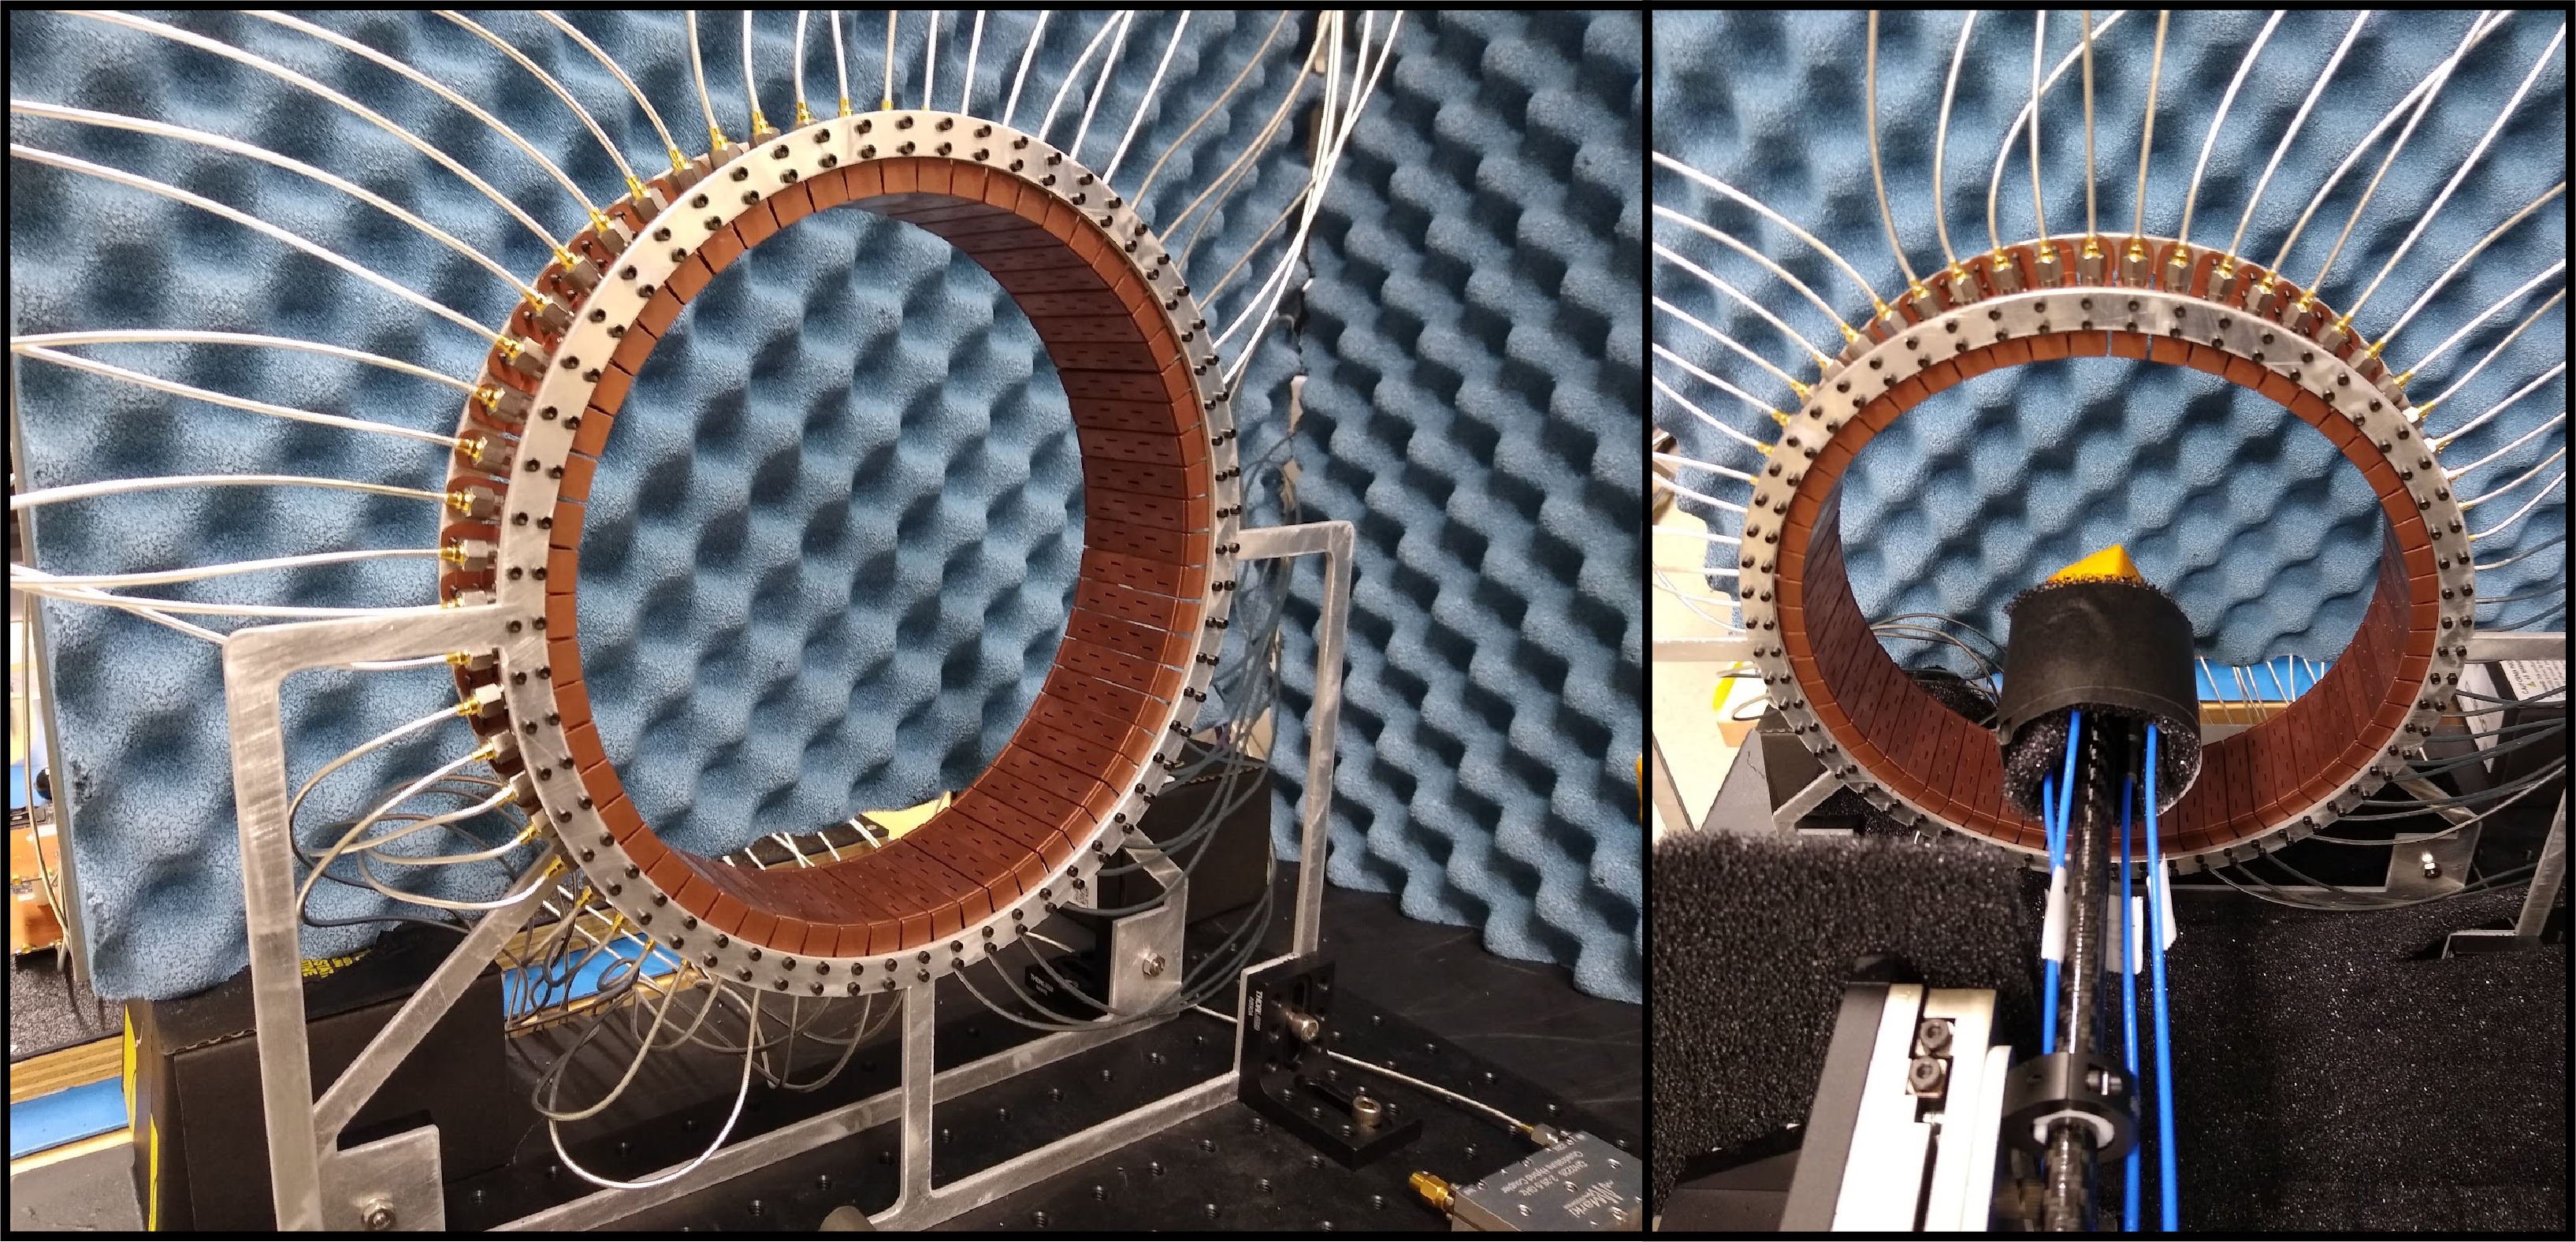
\includegraphics[width=\textwidth]{figs/Chapter-5/230410_jugaad_photo.png}
        \caption{}
        \label{fig:jugaad_photo}
    \end{subfigure}
    \par\medskip
    \begin{subfigure}{0.7\textwidth}
        \centering
        \includegraphics[width=\textwidth]{figs/Chapter-5/230502_jugaad_positioning_system.png}
        \caption{}
        \label{fig:jugaad_positioning_system}
    \end{subfigure}
    \caption{Photos of the prototype FSCD antenna (a), the FSCD array and SYNCA (b), and the translation stages and coordinate system used to position the SYNCA (c).}
    \label{fig:fscd_array_setup}
\end{figure}

The antenna design used in the array is the 5-slot waveguide antenna developed for the FSCD experiment (see Figure \ref{fig:jugaad_antenna_photo}). The antenna is 5~cm long and is constructed out of WR-34 waveguide with a 2.92~mm coax connector located at the center of the antenna. Copper flanges located on both ends of the antenna are used to mount the antenna in the array support structure. The antennas are supported by two circular steel brackets that can be bolted to both ends of the waveguide to construct the circular array (see Figure \ref{fig:jugaad_photo}). The antenna array consists of sixty identical waveguide antennas with a radius of 10~cm. The array  is mounted perpendicular to an optical breadboard surface using a pair of the steel brackets, which provide sufficient space for the coaxial cable connections and allows for easy positioning of the SYNCA antenna. The SYNCA is mounted on the end of a carbon fiber rod attached to a set of manual translation stages, which are used to move the SYNCA antenna to different positions inside the array (see Figure \ref{fig:jugaad_positioning_system}). The stages allow for independent motion in three different axes and can position the SYNCA at radial distances up to 5~cm from the center.

Data acquisition is accomplished using a two-port VNA in combination with a series of microwave switches that allow the VNA to connect to each channel in the array .  The first port of the VNA is connected to the quad-balun chain used to feed the SYNCA (see Section \ref{sec:SYNCA}), and the second port of the VNA connects to a 1P5T microwave switch. The 1P5T switch is connected to four separate 1P16T switch boards that connect directly to the array. The data acquisition is controlled by a python script running on a lab computer which, is connected to the VNA and an Arduino board programmed to control the microwave switches. The script uses the switches to iteratively connect each of the antennas in the array to the VNA, which loads the calibration file for the appropriate channel and performs the measurements for all S-parameters.

Array measurements were performed for the set of SYNCA positions consisting of radial (x-axis) positions from 0 to 50~mm in 5~mm steps and axial (z-axis) positions from 0 to 50~mm in 5~mm steps resulting in 121 array measurements. At each SYNCA position we measured the two-port S-parameter matrix using a linear frequency sweep from 25.1 to 26.1 GHz with 101 discrete frequencies. For each antenna in the array the VNA uses a separate calibration file so that errors arising from path differences in the RF switches are effectively removed. 

\subsubsection{Synthetic Array Setup}

The setup used to perform the synthetic array measurements is shown in Figure \ref{fig:dig-meas-sys}. The notable difference between this setup and the FSCD array setup is that the synthetic array measurements were performed with a waveform generator and digitizer instead of a VNA. However, we are still be able to compare the measured phases of the synthetic array and the relative magnitude of the power, since the digitized signal power is directly proportional to S21. 

The arbitrary waveform generator is configured to produce a 64 MHz sine wave signal that is upconverted to 25.864~GHz using the a mixer and the VNA source configured to output a 25.8~GHz continuous wave. This signal is passed through a filter and fed to the SYNCA quad-balun chain. A single FSCD antenna is positioned 10~cm from the SYNCA and aligned vertically so that the center of the 5-slot waveguide is in the plane of the SYNCA PCB (see Figure \ref{fig:synth_array_photo}). This position corresponds to $z=0$ in Figure \ref{fig:jugaad_positioning_system}. 
\begin{figure}[htbp]
    \centering
    \includegraphics[width=0.5\textwidth]{figs/Chapter-5/230412_IMG_2756.png}
    \caption{A photo of the FSCD antenna and the SYNCA in the synthetic array measurment setup at Penn State.}
    \label{fig:synth_array_photo}
\end{figure}
The SYNCA is rotated in three degree steps to synthesize an antenna array with 120 channels, which is more than could physically fit in a 10~cm radius array, to check of the smoothness of the antenna array radiation pattern. The signals from the FSCD antenna are downconverted using another mixer connected to the VNA source before being digitized at 250~MHz and saved to disk. Several synthetic array measurement scans were performed by using the linear translation stage to change the radial position of the SYNCA. In total eight scans were taken from 0 to 35~mm using a radial position step size of 5~mm.

\subsection{Simulations, Analysis, and Results}

The Locust and CRESana simulation packages utilize the antenna transfer functions to calculate the amount of power that would be received by each antenna in the array from the electric fields produced by a trapped electron. For our VNA array setup the quantity that is directly proportional to this is the S21 matrix element, which indicates the ratio of the power received by an antenna in the array to the amount of power delivered to the SYNCA. Therefore, our analysis will focus on comparing the relative magnitude and phase of the the S21 parameters measured by the VNA as a function of the array channel and the SYNCA position. Additionally, we apply a beamforming reconstruction to the S21 data to evaluate how the summed power and beamforming images change as a function of the position of the SYNCA.

\subsubsection{Simulations}

Simulations for the FSCD array measurements were performed using CRESana, which performs analytical calculations of the EM-fields produced by an electron at the position of the antennas. At each sampled time CRESana computes the electric field vector at the antenna positions, which is projected onto the antenna polarization axis to obtain the copolar electric field. The magnitude of the copolar electric field is then multiplied by a flat antenna transfer function to calculate the voltage signal produced by the antenna. CRESana simulations exploit the flat transfer functions of the FSCD antennas, which allows the electric field to be multiplied by the antenna transfer function rather than performing the full FIR calculation. These calculations produce a voltage time-series for each of the antennas in the array which can be analyzed in terms of the power in each antenna channel and the relative phase between channels to compare to the laboratory measurements.

CRESana was configured to simulate a $90^\circ$ electron in a constant background magnetic field of $\approx0.958$~T to with a kinetic energy of 18.6~keV. These parameters were chosen in order to mimic a possible CRES event near the tritium beta-decay spectrum endpoint in the FSCD experiment. The constant background magnetic field guarantees that the guiding center of the electron is stationary across the duration of the simulation which is consistent with the SYNCA in the laboratory measurements. Simulations were performed with the electron's guiding center at radial positions from 0 to 45~mm in steps of 1~mm and axial positions from 0 to 30~mm in steps of 1~mm. The simulations generated time series consisting of 
8192 samples at 200~MHz for the sixty channel FSCD antenna array geometry.

\subsubsection{Phase Analysis}

\begin{figure}[htbp]
    \centering
    \includegraphics[width=0.7\textwidth]{figs/Chapter-5/230504_cresana_phases.png}
    \caption{The unwrapped phases of signals received by the FSCD antenna array from an electron with a $90^\circ$ pitch angle located in the plane of the antenna array. The data points indicated the phases extracted from simulation and the dashed lines show the model predictions. }
    \label{fig:cresana_simulated_phases}
\end{figure}

The first part of our analysis examines the phases of the signals received by each channel in the antenna array since these features are fundamental to performing a beamforming reconstruction of the array signals as well as constructing accurate matched filter templates. Using simulations we have developed a beamforming phase model that allows us to predict the correct beamforming phases for a specific magnetic trap and assumed electron position. The equation for the model is
\begin{equation}
    \phi_{ij}(t) = \frac{2\pi d_{ij}(t)}{\lambda} + \theta_{ij}(t),
    \label{eq:phase_model_eqn}
\end{equation}
where $d_{ij}(t)$ is distance between the assumed electron position and the antenna position, and $\theta_{ij}(t)$ is the angular separation between the electron and antenna positions. For more details on the components of the phase model see Section \ref{sec:pheno}. In Figure \ref{fig:cresana_simulated_phases} we compare the phases predicted by Equation \ref{eq:phase_model_eqn} to phases extracted from CRESana simulations of an electron located in the plane of the antenna array at a series of radial positions and observe excellent agreement between the model and simulation.

In Figures \ref{fig:jugaad_phase} and \ref{fig:synth_jugaad_phase} we compare the phases measured in the FSCD array setup and the synthetic array setup to the phase model for a set of SYNCA radial positions. The axial position of the SYNCA in both plots is $z=0$~mm, such that the plane of the PCB is aligned with the center of the FSCD antenna. The data shown in Figure \ref{fig:jugaad_phase} corresponds to the S-parameters measured at 25.80~GHz which is the frequency closest to the one used in the synthetic array setup. The different slope and sinusoidal phases exhibited by Figure \ref{fig:jugaad_phase} and \ref{fig:synth_jugaad_phase} reflects differences in the coordinate system for each setup. In general, we see that the phase model predicts the large scale features of the phases quite well, but there are some small scale deviations or errors from the phase model that do not appear to be present in simulation. 
\begin{figure}[htbp]
\centering
\begin{subfigure}{.7\textwidth}
  \centering
  \includegraphics[width=1\textwidth]{figs/Chapter-5/230411_jugaad_measured_phases_z0.png}
  \caption{}
  \label{fig:jugaad_phase}
\end{subfigure}
\par\medskip % force a bit of vertical whitespace
\begin{subfigure}{.7\textwidth}
  \centering
  \includegraphics[width=1\textwidth]{figs/Chapter-5/230411_synthetic_array_measured_phases_z0.png}
  \caption{}
  \label{fig:synth_jugaad_phase}
\end{subfigure}
\caption{Plots of the measured unwrapped phases from the FSCD array (a) and the synthetic array (b) compared to the model predictions for a series of radial positions. The different phases of the sinusoidal phase oscillations in the two plots reflects differences in the coordinate systems of the measurements.}
\label{fig:jugaad_measured_phases}
\end{figure}

We are interested in examining the differences between the data and model more closely, so in Figure \ref{fig:phase-error-curve-comp} we plot comparisons between the phase errors of the synthetic array data and the FSCD array data (labeled JUGAAD in the legend) as a function of the radial position of the SYNCA.
\begin{figure}[htbp]
    \centering
    \includegraphics[width=1\textwidth]{figs/Chapter-5/230414_synthetic_array_phase_error_curves_z0.png}
    \caption{The phase errors between the measurement and model for the synthetic array (blue) and the FSCD array (orange) for a series of radial positions. }
    \label{fig:phase-error-curve-comp}
\end{figure}
Focusing on the trend for the synthetic array phase error data in Figure \ref{fig:phase-error-curve-comp} we see that at $R=0$~mm the phase error forms a relatively smooth curve with the exception of an outlier data point caused by an unintended error in the data acquisition script. Since the position of the SYNCA antenna is stationary at $R=0$~mm, we attribute the observed phase errors to imperfections in the antenna pattern of the SYNCA that cause it to emit a radiation pattern whose phases do not perfectly match the beamforming phase model in Equation \ref{eq:phase_model_eqn}. As the SYNCA is moved away from $R=0$~mm in the synthetic array data we see that the phase error exhibits oscillations whose frequency increases as a function of the radial position of the SYNCA. These oscillations have the appearance of a diffraction pattern, which is particularly obvious for radii $\geq15$~mm, due to the bilateral symmetry of the phase error peaks around $180^\circ$. 

Comparing the phase errors measured in the FSCD array to the synthetic array we see that there is a higher average variance in the phase error. This is best seen by comparing the curves at $R\leq15$~mm where the smooth synthetic array curves are distinct from the relatively noisy FSCD array errors. The extra noise in the FSCD array is most likely caused by differences in the radiation patterns of the antennas that make up the array as well as differences in the transmission lines through the switch network that introduce additional phase errors into the measurement. Since the synthetic array measurements use only a single antenna, these extra error terms are not present, which explains the relatively smoother phase error curves. Despite the extra phase errors in the FSCD array, it is still possible to observe a similar phase error oscillation effect as the SYNCA is moved away from $R=0$~mm.

\begin{figure}[h]
\centering
\begin{subfigure}{.7\textwidth}
  \centering
  \includegraphics[width=1\textwidth]{figs/Chapter-5/230120_synth_array_phase_error_map_z0.png}
  \caption{}
  \label{fig:jugaad_phase_map}
\end{subfigure}
\par\medskip % force a bit of vertical whitespace
\begin{subfigure}{.7\textwidth}
  \centering
  \includegraphics[width=1\textwidth]{figs/Chapter-5/230123_jugaad_phase_error_map_z0.png}
  \caption{}
  \label{fig:synth_jugaad_phase_map}
\end{subfigure}
\caption{Two dimensional plots of the phase errors for the synthetic array (a) and the FSCD (JUGAAD) array (b). In both plots we observe evidence of a similar diffraction pattern with bilateral symmetry, but the FSCD array measurments have an additional phase error contribution from the different antennas and paths through the switch network.}
\label{fig:jugaad_measured_phase_maps}
\end{figure}

The diffraction pattern exhibited by the phase error oscillations is more easily observed by plotting the phase errors in a two-dimensional map, which we do in Figures \ref{fig:jugaad_phase_map} and \ref{fig:synth_jugaad_phase_map}. For the synthetic array data we observe a relatively clear diffraction pattern that emerges as the SYNCA is moved radially. The bilateral symmetry of the diffraction patterns is due to the bilateral symmetry of the circular synthetic array around the translation axis of the SYNCA. A similar pattern is also visible in the FSCD array data although it is obscured by the additional phase error that results from the multi-channel array.

The physical origin of the phase error diffraction pattern is interference effects arising from path-length differences between the individual slots in the FSCD antenna and the SYNCA transmitter. Since we are operating in the radiative near-field of the FSCD antenna, the path length differences between the slots introduces a significant change in the summation of the signals that occurs inside the waveguide, which causes the radiation pattern of the antenna to change as a function of distance. Therefore, when the SYNCA is positioned off-axis the different path-lengths from the SYNCA to each antenna in the array results in different radiation patterns for each of the array antennas producing the observed diffraction pattern. 

This near-field effect is not present in simulations, because in order to simplify the calculations we assume that the far-field approximation can be applied to the FSCD antennas. This means that the radiation pattern and antenna transfer functions are independent of the distance between the transmitter and the receiving antenna. In principle, we can account for these near-field effects with a more detailed simulation of the FSCD antennas either in CRESana or Locust, which would result in an additional term in the beamforming phase model. In the next section we briefly discuss the impact of these near-field effects on the measured magnitude of the signals.

\subsubsection{Magnitude Analysis}

In addition to phase, magnitude is the second component necessary to fully describe the radiation pattern and performance of the antenna array. However, it is not the dominant component from the perspective of beamforming and signal reconstruction. In many cases it is safe to approximate the relative amplitudes of the signals received by each channel as equal with minimal loss in detection efficiency. Therefore, our analysis of the magnitudes from CRESana, the FSCD array, and the synthetic array is less complete and serves mostly to reinforce the conclusions of the phase analysis.

We can use simulations to construct a model that describes the magnitude of the signals received by each channel in the antenna array. By examining the results of simulations or by analyzing the Li\'{e}nard-Wiechert equation one can show that radiation pattern from a $90^\circ$ pitch angle electron in a magnetic field is omni-directional. Therefore the relative magnitudes of the signals received by each channel will be determined by the free-space power loss, which is proportional to the inverse distance between the assumed electron position and the antenna. A consequence of this is that the signals produced in the array for electrons off the central axis will have larger amplitudes for the antennas closer to the electron compared to those which are further away. In Figure \ref{fig:cresana_mags} we plot the amplitudes of the signals received by each antenna in the array from an electron located at a series of radial positions.
\begin{figure}[htbp]
    \centering
    \includegraphics[width=0.7\textwidth]{figs/Chapter-5/230508_cresana_mags.png}
    \caption{The amplitude of the signals from CRESana for the FSCD array from a $90^\circ$ electron. As the electron is moved from $R=0$ the signals begin to have unequal amplitudes depending on the distance from the electron to the antenna.}
    \label{fig:cresana_mags}
\end{figure}

We expect to see a similar trend in the signal magnitudes in both the FSCD and synthetic arrays. In Figure \ref{fig:jugaad_synth_mag_curve_comp} we plot the normalized signal magnitudes extracted from the VNA and digitizer measurements for a series of radial SYNCA positions. We use the data collected at the SYNCA axial position of $z=0$~mm for both the FSCD and synthetic arrays and show the S-parameters measured by the VNA at 25.86~GHz. A complication with these measurements is that the radiation pattern of the SYNCA is not perfectly omni-directional, which causes the measured magnitudes at $R=0$~mm to diverge from the perfectly flat behavior exhibited by electrons.
\begin{figure}[htbp]
    \centering
    \includegraphics[width=1\textwidth]{figs/Chapter-5/230412_jugaad_mag_curves_z0.png}
    \caption{The normalized magnitudes of the S21 parameters measured in the FSCD (orange) and synthetic array (blue) setups. The dominant observed behavior as a function of radius is the increase in the number of magnitude peaks, which was noted in the phase error curves. There does not appear to be a strong change in the relative amplitude of a group of antennas as predicted by CRESana.}
    \label{fig:jugaad_synth_mag_curve_comp}
\end{figure}
As the SYNCA is moved away from $R=0$~mm in the synthetic array we observe a similar increase in the number of magnitude peaks that we would expect in a diffraction pattern, though this trend is less obvious than the phase data. Noticeably, there does not appear to be a set of channels with disproportionately larger amplitude at large $R$, which would be expected based on the trend from simulation. 

\begin{figure}[htbp]
\centering
\begin{subfigure}{.7\textwidth}
  \centering
  \includegraphics[width=1\textwidth]{figs/Chapter-5/230120_synth_array_signal_amplitude_map_z0.png}
  \caption{}
  \label{fig:synth-jugaad-mag-map}
\end{subfigure}
\par\medskip % force a bit of vertical whitespace
\begin{subfigure}{.7\textwidth}
  \centering
  \includegraphics[width=1\textwidth]{figs/Chapter-5/230123_jugaad_magnitude_map_z0.png}
  \caption{The two-dimensional maps showing the diffractive pattern exhibited by the FSCD and synthetic array signal magnitudes.}
  \label{fig:jugaad-mag-map}
\end{subfigure}
\caption{}
\label{fig:measured-mag-map-comp-jugaad}
\end{figure}

Comparing the magnitudes of the synthetic array to the FSCD array in Figure \ref{fig:jugaad_synth_mag_curve_comp} we see that there is a similar amount of variability in the magnitudes at $R=0$~mm, although there is potentially more small scale error in the magnitude curve caused by channel differences in the FSCD array. We observe a similar trend in the number of magnitude error peaks in the FSCD array data to the synthetic array data, which mirrors the diffraction effect observed in the phase data. The diffraction effect can be visualized more clearly by plotting a similar two-dimensional map of the magnitudes (see Figure \ref{fig:measured-mag-map-comp-jugaad}).

Observing a similar diffractive pattern in the signal magnitudes as a function the SYNCA position reinforces our conclusions from the phase analysis that near-field effects are having a significant impact on the radiation pattern of the FSCD array. These near-field effects lead to changes in the magnitude and phase of the radiation pattern of the FSCD antenna as a function of distance. If left uncorrected these errors reduce detection efficiency by causing power loss in the beamforming or matched filter reconstruction due to phase mismatch. We explore the impact of these phase and magnitude errors on beamforming in the next section.

\subsubsection{Beamforming Characterization}
\label{sec:jugaad_bf_analysis}

The errors in the magnitude and phase of the FSCD array radiation pattern lead to errors in the signal reconstruction. For example, a matched filter reconstruction requires accurate knowledge of the relative phases and magnitudes of the signals in each channel to achieve optimal performance. Uncorrected errors here leads to mismatch between the template and signal, which reduces detection efficiency and introduces uncertainty in the parameter estimation. In this section, we analyze the beamformed signal amplitude as a function of the position of the SYNCA to quantify the impact of the phase and magnitude errors on signal reconstruction. Because of the imperfections in the SYNCA source, it is inappropriate to directly compare the beamformed signal amplitude of the FSCD array or synthetic array. Such a comparison would not allow us to disentangle losses that occur because of the antenna array from those that occur because of the source. Therefore, we focus on comparing the beamforming of the FSCD array to the synthetic array.

\begin{figure}[htbp]
    \centering
    \begin{subfigure}[b]{0.48\textwidth}
        \includegraphics[width=1\textwidth]{figs/Chapter-5/230414_z00r15_synth_beamform.png}
        \caption{}
        \label{fig:synth-jugaad-bf-image}
    \end{subfigure}
    \hfill
    \begin{subfigure}[b]{0.48\textwidth}
        \includegraphics[width=1\textwidth]{figs/Chapter-5/230414_z00r15_jugaad_beamform_mean.png}
        \caption{}
        \label{fig:jugaad-bf-image}
    \end{subfigure}
    \hfill
    \caption{Beamforming images from the synthetic array (a) and FSCD array (b) setups with the SYNCA positioned 15~mm off the central axis. In both images we see a clear maxima that corresponds to the true SYNCA position. However, in the FSCD array there is an additional faint peak located at the opposite position of the beamforming maximum. This additional peak is the mirror of the true peak and is the result of reflections between antennas in the FSCD array.}
    \label{fig:measured-bf-images}
\end{figure}

Our first method of comparison is to analyze the images generated by applying the beamforming reconstruction specified in Section \ref{sec:chap4-dig-bf} to the FSCD and synthetic array data (see Figure \ref{fig:jugaad-bf-compare}). We use a beamforming grid consisting of a square $121\times121$ grid spanning a range of -60-mm to 60~mm in the x and y dimensions. The beamforming images formed from the synthetic array produces a three-dimensional matrix where each grid position contains a summed time series. We form a single beamforming image from this matrix by taking the average over the time dimension. Applying beamforming to the FSCD array data also produces a three-dimensional matrix, but in this case each grid position contains a summed frequency series produced by the VNA sweep. In order to generate a clearer beamforming image we average over the entire frequency sweep.

There is a clear difference between the synthetic and FSCD array beamforming images, which is the additional faint beamforming maxima located directly opposite the maxima corresponding to the SYNCA position. The images in Figure \ref{fig:measured-bf-images} were generated with data collected at a SYNCA radial position of 15~mm, which agrees well with the observed beamforming maximum in both images. We observe that the faint beamforming peak is located directly opposite of the true beamforming maximum similar to a mirror image. Therefore, the origin of this additional feature appears to be reflections between the two sides of the circular antenna array that are not present for the synthetic array since only a single physical antenna is used.

\begin{figure}[htbp]
    \centering
    \begin{subfigure}[b]{0.48\textwidth}
        \includegraphics[width=1\textwidth]{figs/Chapter-5/230509_synth_beamform_amplitude.png}
        \caption{}
        \label{fig:synth-jugaad-bf-amp}
    \end{subfigure}
    \hfill
    \begin{subfigure}[b]{0.48\textwidth}
        \includegraphics[width=1\textwidth]{figs/Chapter-5/230509_fscd_array_beamform_amplitude.png}
        \caption{}
        \label{fig:jugaad-bf-amp}
    \end{subfigure}
    \hfill
    \caption{A comparison of the maximum signal amplitude obtained by beamforming to the signal amplitude obtained with an ideal summation as a function of the radial position of the SYNCA. The amplitudes for the synthetic array are shown in (a) and the FSCD array are shown in (b). In both setups we observe that the signal amplitudes obtained from beamforming are smaller than the signal amplitude that could be attained with the ideal summation without phase mismatch.}
    \label{fig:measured-bf-amp}
\end{figure}

From the beamforming images we extract the maximum amplitude, which we plot as a function of the radial position of the SYNCA (see Figure \ref{fig:measured-bf-amp}). The phase errors we observed in the FSCD and synthetic arrays leads to power loss at the beamforming stage due to phase mismatches between the signals at different channels. This power loss can be quantified by comparing the signal amplitude obtained from beamforming to the amplitude which would be obtained from an ideal summation. We perform the ideal summation by phase shifting each array channel to the same phase and then summing. The comparison between the beamforming and ideal sums is shown in Figure \ref{fig:measured-bf-amp}, where we observe that both the synthetic and FSCD arrays experience power losses from the beamforming summation. 

\begin{figure}[htbp]
    \centering
    \includegraphics[width=.6\textwidth]{figs/Chapter-5/230509_beamformed_idealsum_ratio_compare.png}
    \caption{The ratio of the beamforming signal amplitude to the ideal signal amplitude for the FSCD and synthetic arrays. We see that the FSCD array has a larger power loss from phase error compare to the synthetic array which indicates that calibration errors associated with the multiple channels as well as reflections are impacting the signal reconstruction. }
    \label{fig:jugaad-synth-bf-amp-ratio}
\end{figure}

The beamforming power loss can be quantified using the ratio of the beamforming to ideal signal amplitudes. Computing this ratio as a function of SYNCA radial position radius for the FSCD and synthetic arrays we find that the FSCD array has a uniformly smaller beamforming amplitude ratio, which means that the FSCD array has a larger beamforming power loss (see Figure \ref{fig:jugaad-synth-bf-amp-ratio}). The primary contributions to the beamforming power loss in the synthetic array are phase errors from the SYNCA and phase errors from the FSCD antenna near-field. Both of these phase errors contribute to beamforming losses in the FSCD array, but there are clearly additional phase errors in the FSCD array measurements contributing to the smaller ratio. Two potential error sources include phase differences in the different antenna channels that could not be corrected by calibration as well as reflections between antennas in the array. The total effect of these additional phase errors is to reduce the beamforming amplitude ratio by about 5\% from the beamforming ratio of the synthetic array. Therefore, we estimate that if no effort is made to correct these phase errors in an FSCD-like experiment, then we expect approximately a 10\% total signal amplitude loss from a beamforming signal reconstruction. 

\subsection{Conclusions}

The estimated power loss of a beamforming reconstruction obtained from this analysis provides valuable inputs to sensitivity calculations of a FSCD-like antenna array experiment to measure the neutrino mass, since it helps to bound systematic uncertainties from the antenna array and reconstruction pipeline. This power loss lowers the estimated detection efficiency of the experiment since some of the signal power is lost due to improper combining between channels and also increases the uncertainty in the electron's kinetic energy by contributing to errors in the estimation of the electron's cyclotron frequency. 

If these reconstruction losses prove unacceptable there are steps that can be taken to mitigate their effects. Some examples include the development of a more accurate antenna simulation approach that can reproduce the observed near-field interference patterns of the FSCD antennas and the implementation of a calibration approach that allows for the relative phase delays of the array to be measured without changing or disconnecting the antenna array configuration. 